\section{Attitude} \label{Ch:Attitude}
The attitude of a spacecraft can be defined qualitatively as how the spacecraft
is oriented in inertial space, and how that orientation changes in time. GMAT
has the ability to model the orientation and rate of rotation of a spacecraft
using several different mathematical models.  Currently, GMAT assumes that a
spacecraft is a rigid body.

There are many ways to quantitatively describe the orientation and rate of
rotation of a spacecraft, just like there are many ways we can quantitatively
describe an orbit state. Let's define any set of numbers that can uniquely
define the spacecraft attitude as an \emph{attitude parameterization}.  GMAT
allows its users to employ several common attitude parameterizations including
quaternions, Euler angles, the Direction Cosine Matrix (DCM) or Attitude Matrix
\textbf{A}, Euler angle rates, and the angular velocity vector. Given an initial
attitude state, GMAT can propagate spacecraft attitude using one of several
kinematic or dynamic attitude propagation models.

Our notation will be based on a compromise that spans multiple disciplinary
fields, from astrodynamics and aircraft flight simulation to computer graphics,
and is informed by the AIAA and CCSDS standards.  We want a consistent
definition in the inner core algorithms of GMAT combined with the capability of
translating internal variables into interface variables that are easy for users
to understand and work with.  For example, if a user wishes to visualize the
attitude of a specific mission spacecraft using quaternions extracted from real
world telemetry, GMAT should be flexible enough for that user to define all four
quaternion components, their locations with respect to each other, and their
numerical signs.  The user should also be able to specify the two reference
frames the attitude parameterization is relating, and the direction the attitude
parameters take a transformation.  In other words, following the CCSDS standard,
the user should be able to specify which is the ``from" frame and which is the
``to" frame.

We should also point out that the parameters presented in this document can
describe not only the ``transformation" of a vector between two reference frames,
but also the ``rotation" of a vector from one orientation to another in the same
reference frame.  The literature uses the definition of ``transformation" and
``rotation" quite liberally, and a detailed search has found little agreement on
terminology and notation.  Almost all authors agree that the components of the
3$\times$3 matrix relating vectors to each other are ``Direction Cosines".  They
are the dot products of the basis axes unit vectors of one reference frame with
the basis axes unit vectors of the other reference frame.  They are the cosines
of the angles between each of the basis axes.

For now it is suggested that the matrix we use to transform or rotate vectors be
labeled \textbf{R} to remain consistent with the mathematical development
earlier in this specification in Chapter~\ref{Ch:CoordinateSystems}.  The
3$\times$3 matrix \textbf{R} will relate various reference frames to each other
and can be used to rotate vectors between frames such as in the FK5 reduction
process.  Meanwhile, if we wish to explicitly model the attitude or orientation
of a spacecraft, we can represent this with the 3$\times$3 matrix \textbf{A}.
The letter brings the word ``Attitude" to mind, and is used by several well known
attitude dynamics authors including Landis Markley who wrote the
"Parameterization of the Attitude" section of ``Spacecraft Attitude
Determination and Control" by James R. Wertz, a very popular text in the field.
To be consistent with Chapter~\ref{Ch:CoordinateSystems}, we should specify the
direction of the transformation with additional notation.

Meanwhile, if we intentionally keep our notation as clutter free as possible,
the definition of \textbf{A} will be as follows.

\begin{equation}
    \textbf{ b = Ar}
    \label{Eq:FundamentalAMat}
\end{equation}

In this equation \textbf{b} is a vector in the spacecraft body frame, and
\textbf{r} is a vector in the reference frame.  The attitude matrix \textbf{A}
transforms vectors from the reference frame to the body frame.

The human mind has some difficulty visualizing the orientation of a spacecraft
when presented with the nine component attitude matrix.  Likewise, it is
difficult to know if an aircraft or spacecraft is ``upside-down" given the four
components of a quaternion vector.  For human interface purposes, the attitude
descriptor of choice is the set of three Euler Angles, such as the classic
``roll", ``pitch", and ``yaw".  The CCSDS specification avoids mentioning the DC
matrix altogether.  Meanwhile, GMAT will use it as an intermediate form of
attitude parameterization when transforming from internal attitude propagation
equations using quaternions, and human interpretable Euler Angles.  GMAT will
also use it for both Coordinate System Fixed and Spinning Spacecraft modes of
attitude propagation.

In this chapter, we discuss the attitude parameterizations supported in GMAT,
and how to convert between the different types.  We discuss the internal state
parameterization that GMAT uses.  Next we investigate the types of attitude
modes in GMAT and discuss in detail how GMAT propagates the spacecraft attitude
in all of the Kinematic and Dynamic attitude modes.  We conclude the chapter
with a discussion of how GMAT converts between different attitude
parameterizations.

\subsection{Attitude Propagation}

Given a set of initial conditions that define the attitude, GMAT can propagate
the attitude using several methods.  Currently, GMAT supports both Kinematic
attitude and Dynamic attitude propagation.  In Kinematic mode, the attitude is
defined by describing the desired orientation with respect to other objects such
as spacecraft or celestial bodies.  With this information, GMAT can calculate
the required attitude to satisfy the desired geometrical configuration.  In
Dynamic mode, the user must also supply spacecraft body inertial mass properties,
and tell GMAT how to apply torques dynamically to the spacecraft.  With these
conditions specified, GMAT will numerically integrate quaternion attitude
equations of motion combined with Euler's moment equations.  The resulting
attitude motion will display basic physics-based phenomena such as precession
and nutation.  Dynamic mode will allow a user to model the implementation of
attitude control laws, as well as the effects of asymmetric propellant mass
depletion and dynamic spacecraft component articulation.  It will also
eventually support the modeling of attitude perturbations such as Gravity
Gradient, Aerodynamic Drag and Solar Photon Pressure Torques, and spacecraft
magnetic interaction with planetary magnetic fields.  This section presents the
different Kinematic and Dynamic attitude modes, and how GMAT calculates the
attitude state in each mode.  Let's begin by looking at the internal attitude
state representations and how the user can define initial conditions.

\vspace{- .1 in} \subsubsection{Internal State Representation and Attitude
Initial Conditions}

As mentioned in the introduction, certain attitude parameterizations are more
useful for attitude propagation, while other attitude parameterizations are
more intuitive for providing attitude initial conditions or output.  GMAT uses
different internal parameterizations of the attitude depending on the attitude
mode.  The type of parameterization is chosen to make the attitude propagation
algorithms natural and convenient.  For the Kinematic modes, GMAT uses the
Direction Cosine Matrix (DCM) or "Attitude" matrix that represents the rotation
from the inertial reference frame to the body frame.  The notation for the
Attitude matrix, including the direction of the rotation it parameterizes is
\textbf{A}$_{BI}$.  The subscripts denote the direction of the rotation from
Inertial to Body frames.  For Dynamic mode, six degree of freedom (6DOF)
attitude propagation, GMAT uses the quaternion that represents the rotation from
the inertial reference frame to the body frame.  The notation for the quaternion,
including the direction of the rotation it parameterizes, is
\textbf{\emph{q}}$_{BI}$.  Once again, the subscripts denote the direction of
the rotation from Inertial to Body frames.  GMAT uses the angular velocity of
the body with respect to the inertial frame, expressed in the body frame,
$\{\boldsymbol\omega_{IB}\}_B$, as the rate portion of the state vector.

For convenience, the user can choose a coordinate system in which to define the
initial attitude state.  Let's call this system $\mathcal{F}_i$.  The user can
define the initial attitude with respect to $\mathcal{F}_i$ using Euler angles,
the DCM or attitude matrix \textbf{A}, or quaternions.  The user can define the
body rate with respect to $\mathcal{F}_i$ by defining the angular velocity in
$\mathcal{F}_i$, $\{\boldsymbol\omega_{IB}\}_i$, by defining the angular
velocity in the inertial frame as measured in body coordinates
$\{\boldsymbol\omega_{IB}\}_B$ or by defining the Euler angle rates.  Note that
not all attitude modes require these three pieces of information.  The specific
inputs for each attitude mode are discussed below, along with details about how
attitude propagation is performed in each mode.

\subsubsection{Kinematic Attitude Propagation}

The Kinematic attitude mode allows a user to define a geometrical configuration
based on the relative position of a spacecraft with respect to other spacecraft
or celestial bodies, and with respect to different coordinate systems.  In
Kinematic mode, GMAT does not integrate the attitude equations of motion, but
rather calculates the attitude based on the geometrical definition provided by
the user.  There are two Kinematic modes to choose from.  These are Coordinate
System Fixed and Spinning Spacecraft.  The different modes allow the user to
conveniently define the spacecraft attitude depending on the type of attitude
profile needed for a specific mission.  To begin, let's look at how GMAT
calculates the attitude state in the Coordinate System Fixed attitude mode
(CSFixed).

\subsubsection{Coordinate System Fixed Mode}

In the CSFixed attitude mode, the user specifies a coordinate system $\mathcal{F}_i$ in which to fix the attitude.
$\mathcal{F}_i$ can be any of the default coordinate systems or any user defined
coordinate system. GMAT calculates the attitude matrix of $\mathcal{F}_i$ using the
following equation.
%
\begin{equation}
    \mathbf{A}_{BI} = \mathbf{R}_{iI}
    \label{Eq:CSFixedRotationMatrix}
\end{equation}
%
$\mathbf{R}_{iI}$ is the DCM matrix relating $\mathcal{F}_I$ to $\mathcal{F}_i$
and GMAT knows how to calculate this matrix for all allowable $\mathcal{F}_i$.
For details on the calculation of this matrix for all coordinate systems in GMAT
see Ch.~\ref{Ch:CoordinateSystems}. To calculate $\{\mathbf{\boldsymbol\omega}_{IB}\}_B$, we start from Euler's
equation:
%
\begin{equation}
    \dot{\mathbf{A}}_{BI} = -\{\mathbf{\boldsymbol\omega^\times}_{IB}\}_B\mathbf{A}_{BI}
    \label{Eq:CSFixedKinematics}
\end{equation}
%
% Note from Dunn:  We want the "where" statement below to stay above the
% equation and not be orphaned on the preceding page.  Adding \\* makes the
% "where" line stay with the equation below.  Then we have to add the [0.5cm]
% AND skip the white line between this line and the \begin{equation} command so
% the vertical white space looks good.  If we change to 10 pt when integrating
% back into Steve's main document, the [0.5cm] command might need a tweak.
where\\*[0.5cm]
%
\begin{equation}
    \{ \mathbf{\boldsymbol\omega^\times}_{IB}\}_B\hspace{0.082cm}\equiv
        \begin{bmatrix}
                 0      & -\omega_{3} &  \omega_{2} \\
             \omega_{3} &      0      & -\omega_{1} \\
            -\omega_{2} &  \omega_{1} &      0
        \end{bmatrix}
    \equiv \hspace{0.082cm}\boldsymbol \Omega
    \label{Eq:OmegaCrossMatrix}
\end{equation}
%
and $\{\mathbf{\boldsymbol\omega}_{IB}\}_B$ is the skew symmetric angular
velocity ``cross product matrix" of $\mathcal{F_B}$ with respect to
$\mathcal{F}_I$, expressed in $\mathcal{F}_B$.  Solving Equation
\ref{Eq:CSFixedKinematics} for $\{\mathbf{\boldsymbol\omega}_{IB}^\times\}_B$
we obtain
%
\begin{equation}
    \{\mathbf{\boldsymbol\omega^\times}_{IB}\}_B =  -\dot{\mathbf{A}}_{BI}\mathbf{A}_{BI}^{T}
    \label{Eq:CSFixedKinematics2}
\end{equation}
%
where 
%
\begin{equation}
     \dot{\mathbf{A}}_{BI} = \dot{\mathbf{R}}_{iI}
    \label{Eq:CSFixedKinematics2}
\end{equation}
%Taking the derivative of Equation \ref{Eq:CSFixedRotationMatrix} with respect to
%time yields
%%
%\begin{equation}
%    {\mathbf{\dot A}_{BI}} = \mathbf{A}_{Bi}{\mathbf{\dot R}_{iI}}
%    \label{Eq:CSFixedTimeDerivative}
%\end{equation}
%%
%because by definition, for the CSFixed mode,
%$ \mathbf{\dot A}_{Bi} = \mathbf{0}$.
%Substituting Eq. \ref{Eq:CSFixedTimeDerivative} into
%Eq. \ref{Eq:CSFixedKinematics2} we obtain
%%
%\begin{equation}
%    \{\mathbf{\boldsymbol\omega^\times}_{IB}\}_B =  -\mathbf{A}_{Bi}{\mathbf{\dot R}_{iI}} \mathbf{A}_{BI}^{T}
%    \label{Eq:CSFixedKinematics3}
%\end{equation}
%%
%where $\mathbf{A}_{Bi}$ is known from user input, and $\mathbf{A}_{BI}$ is known
%from Eq. \ref{Eq:CSFixedRotationMatrix}.  GMAT knows how to calculate
%$\mathbf{\dot{R}}_{iI}$ for all allowable $\mathcal{F}_i$ and details are contained
%in Ch.~\ref{Ch:CoordinateSystems}.  Next we would like to get the angular
%velocity vector $\{\mathbf{\boldsymbol\omega}_{IB}\}_B$ in terms of the
%components of the 3$\times$3 cross product matrix in the middle of
%Eq. \ref{Eq:OmegaCrossMatrix}.  This matrix, in symbol notation also shows up on
%the left hand side of Eq. \ref{Eq:CSFixedKinematics3}.
%%
%% Note - Dunn discovered, through trial and error, that you can't add white lines
%% between matrix components in the equation below to enhance readability.  LaTeX
%% actually crashes.  But you can add a % comment to create spacing.
%\begin{equation}
%	\{\boldsymbol \omega_{IB}\}_{B} =
%        %
%        \begin{bmatrix}
%            \omega_{1} \\
%            \omega_{2} \\
%            \omega_{3}
%        \end{bmatrix} = \hspace{0.082cm}
%        %
%        \begin{bmatrix}
%            \Omega_{32} \\
%            \Omega_{13} \\
%            \Omega_{21}
%        \end{bmatrix}
%        %
%    \label{Eq:OmegaComponents}
%\end{equation}
%%
%Each of the three components of the angular velocity vector, measured in the
%spacecraft body frame, can be found in the cross product matrix defined in
%Eq. \ref{Eq:OmegaCrossMatrix}.  The subscripts on the right hand side of
%Eq. \ref{Eq:OmegaComponents} tell us where to find these components after
%multiplying the three 3$\times$3 matrices on the right hand side of
%Eq. \ref{Eq:CSFixedKinematics3}.


\subsubsection{Spinning Spacecraft Mode}

In spinning spacecraft mode, GMAT propagates the attitude by assuming the spin
axis direction is fixed in inertial space.  The spacecraft attitude at some time,
$t$, is kinematically propagated from the attitude initial conditions.
The user defines the initial attitude with respect to $\mathcal{F}_i$ by providing $\mathbf{A}_{BI}(t_o)$ or an equivalent
parameterization that is then converted to the Attitude matrix.  The user also
provides the angular velocity of the body axes with respect to the inertial axes
expressed in $\mathcal{F}_i$, $\{\boldsymbol\omega_{IB}\}_i$.  

To calculate $\mathbf{A}_{BI}(t)$ where $t$ is an arbitrary epoch,
we begin by calculating $\mathbf{A}_{B_{o}I}$, understanding that
$\mathbf{A}_{B_{o}I} = \mathbf{A}_{BI}(t_o)$.  We calculate
$\mathbf{A}_{B_{o}I}$ using
%
\begin{equation}
    \mathbf{A}_{B_{o}I} =  \mathbf{A}_{Bi}\mathbf{R}_{iI}(t_o)
    \label{Eq:ABoI}
\end{equation}
%
where $\mathbf{A}_{Bi}$ comes from user provided data, and
$\mathbf{R}_{iI}(t_o)$ is calculated by GMAT and is dependent upon
$\mathcal{F}_i$.  See Ch.~\ref{Ch:CoordinateSystems} for details on how GMAT
calculates $\mathbf{R}_{iI}$ for all allowable coordinate systems in GMAT.

Before calculating $\mathbf{A}_{BI}(t)$ we must determine the spin axis in the
body frame, $\{\boldsymbol\omega_{IB}\}_B$.  If the user has chosen to provide
the angular velocity vector in body frame coordinates, then we already have what
we need.  Otherwise, the user provides $\{\boldsymbol\omega_{IB}\}_i$.
In spinning mode we assume the rotation rate magnitude is constant and also that
the spin axis direction is constant in inertial space.  This assumption is only
realistic if the angular velocity is aligned with either the maximum or minimum
primary axis of moment of inertia in the spacecraft body reference frame.  If
angular velocity is aligned with the axis of minimum moment of inertia, then we
must also assume there is an active attitude control system holding it there.
If there is no control system, and the spacecraft dissipates rotational kinetic
energy (all real bodies will) then the direction of the angular velocity vector
will migrate slowly until it is aligned with the axis of maximum moment of
inertia.  Understanding these assumptions we can state
$\{ \boldsymbol\omega_{IB} \}_B (t)$ $ = \{\boldsymbol\omega_{IB} \}_B (t_o) =
\{ \boldsymbol\omega_{IB} \}_B$.  We can find the spin axis in the body frame
(if we need to) using $\mathbf{A}_{Bi}$ as follows
%
\begin{equation}
    \{ \boldsymbol\omega_{IB}\}_B = \mathbf{A}_{Bi} \{ \boldsymbol\omega_{IB}\}_i
    \label{Eq:AngularVelocityBody}
\end{equation}
%
Once calculated, GMAT saves the parameters $\mathbf{A}_{B_{o}I}$ and
$\{\boldsymbol\omega_{IB}\}_B$ for use in calculating the attitude and rate at
other epochs.

GMAT calculates $\mathbf{A}_{BI}(t)$ using the Euler axis/angle to Attitude
matrix conversion algorithm  in Sec.\ref{Sec:AttitudeParameterizations}. The
Euler axis is simply the unitized angular velocity vector or,
%
\begin{equation}
    \mathbf{a} =   \frac{  \{ \boldsymbol\omega_{IB} \}_B  }{\omega_{IB} }
\end{equation}
%
where
%
\begin{equation}
    \omega_{IB} = \| \{\boldsymbol{\omega}_{IB} \}_B \|
\end{equation}
%
\newpage
The Euler angle $\phi$ is calculated using
%
\begin{equation}
    \phi(t) = \omega_{IB}(t -t_o)
\end{equation}
%
where $t$ is the current epoch, and $t_o$ is the spacecraft's initial epoch.
Let's define the Attitude matrix that results from the Euler axis/angle to
Attitude matrix conversion algorithm using $\mathbf{a}$ and $\phi(t)$, as
$\mathbf{A}_{BB_{o}}(t)$.  We can calculate $\mathbf{A}_{BI}(t)$ using
%
\begin{equation}
    \mathbf{A}_{BI}(t) =
    \mathbf{A}_{BB_{o}}(t)\mathbf{A}_{B_{o}I}
\end{equation}
%
To summarize, in spinning mode the user provides $\mathbf{A}_{Bi}$ and
$\{ \boldsymbol\omega_{IB}\}_i$ or $\{ \boldsymbol\omega_{IB}\}_B$.  GMAT
assumes that that the spin axis direction is constant in both inertial and body
space, and uses the Euler axis/angle method to propagate the attitude to find
$\mathbf{A}_{BI}$.  Now let's look at dynamic attitude propagation in GMAT.


\subsubsection{Dynamic Attitude Propagation}
In Dynamic mode, GMAT propagates quaternion attitude equations of motion along
with Euler's moment equations.  This allows the user to provide detailed mass
moment of inertia properties, and to model spacecraft attitude control and
environmental perturbing torques.  The resulting numerically integrated attitude
will exhibit basic dynamics properties such as precession and nutation.
Detailed tracking of the dynamic inertia tensor will also allow the user to
properly model the effect on the attitude trajectory of propellant mass
depletion, articulation of various components, and implementation of attitude
control laws.  For modes where control laws cause the spacecraft to slew to a
targeted pointing direction, GMAT will model line of sight angular acceleration,
deceleration, overshoot, settling, and drift behavior.  There are several
Dynamic modes to choose from.  The different modes allow the user to
conveniently define the spacecraft attitude and controlled pointing depending on
the type of attitude profile needed for a specific mission.  To begin, let's
look at how GMAT calculates the attitude state in the simplest possible dynamic
mode, Rigid Torque Free attitude mode (RigidTorqueFreeQuat).\\*[0.1cm]
%
\vspace{-0.2 in}
\begin{figure*}[htb]
    \begin{center}
    \includegraphics[width=0.8\textwidth]{Images/QuaternionX42DefB&W}
    \caption{ Euler Axis and Angle} \label{fig:EulerAxisAndAngle}
    \end{center}
\end{figure*}
%
\subsubsection{Rigid Torque Free (Quaternion) Mode}
The fundamental equations of attitude motion run most efficiently using the four
component quaternion.  There are equations of motion for Euler Angles, but these
have singularities that cause problems in implementation.  There are also
equations of motion for the nine components of the Attitude matrix.  Numerically
integrating nine equations for the Attitude matrix is not as efficient as four
equations for the quaternion.  The quaternion is the most popular attitude
parameterization in use today for propagating attitude using numerical
integration schemes.  Let's begin by defining the quaternion.

As shown above in Figure \ref{fig:EulerAxisAndAngle}, any spacecraft attitude
can be described as the rotation about a single axis via a fixed angle from an
inertial frame orientation to the current body orientation.  The single axis is
called the Euler Axis, and the angle is the Euler Angle.  In the figure, the
Euler Axis is given the vector label $\vec{e}$.  This is not the same as
the three Euler Angles used as another of our attitude parameterizations.  We
will use the CCSDS Attitude Data Message standard to define the GMAT quaternion.
The definition is based on the Euler Axis/Angle parameterization and is
%
\begin{equation}
	\boldsymbol q \equiv
        %
        \begin{bmatrix}
            q_1 \\
            q_2 \\
            q_3 \\
            q_c
        \end{bmatrix}
        %
        \equiv %\hspace{0.082cm}
        %
        \begin{bmatrix}
            \mathbf{q} \\
            q_c \\
        \end{bmatrix}
        %
        \equiv %\hspace{0.082cm}
        %
        \begin{bmatrix}
            \mathbf{a}_1 \sin \frac{\phi}{2} \\
            \mathbf{a}_2 \sin \frac{\phi}{2} \\
            \mathbf{a}_3 \sin \frac{\phi}{2} \\
            \cos \frac{\phi}{2} \\
        \end{bmatrix}
        %
    \label{Eq:QuaternionDefinition}
\end{equation}
%
where $\mathbf{a}_1$, $\mathbf{a}_2$, and $\mathbf{a}_3$ are components of the
unit vector aligned with the Euler Axis or $\mathbf{\hat{a}}$.  This unit vector
is shown near the spacecraft center of mass in Figure \ref{fig:EulerAxisAndAngle}.
In Eq.~\ref{Eq:QuaternionDefinition} the Euler Angle is denoted using the symbol
 $\phi$.  There are actually two possible values of $\phi$, since the rotation
shown in Figure \ref{fig:EulerAxisAndAngle} can be the long way around or the
short way around.  The two possible values will add to $360\,^{\circ}$.  Our
definition of quaternions assumes the smaller angle.

The subscript ``c" on the fourth component of the quaternion comes from the
CCSDS standard and most likely stands for ``cosine".  The CCSDS has cleverly
avoided specifying whether the cosine ``scalar" component should be placed
before or after the vector component.  This standard has thus eliminated the
confusion of which component of the quaternion should be defined as $q_1$ and
which as $q_4$.  The CCSDS standard does place its initial definition for $q_c$
after the definitions for $q_1$, $q_2$, and $q_3$.  This lets us stack the four
components in the vector shown in the second part of the definition in
Eq.~\ref{Eq:QuaternionDefinition}.  If $q_4$ were substituted for $q_c$, we would
have Landis Markley's definition from the ``Parameterization of the Attitude"
section in ``Spacecraft Attitude Determination and Control" by Wertz.  The third
part of the definition above shows the 3$\times$1 vector component of the
quaternion as a single symbol $\mathbf{q}$, placed above $q_c$ to form a second
4$\times$1 matrix or vector.  This also parallels Markley's definition and will
conveniently fit into the GMAT equations relating quaternions to the Attitude
matrix shown later in this section.  Note that for the final part of the
definition in Eq. \ref{Eq:QuaternionDefinition}, the CCSDS standard uses
$\mathbf{e}$ to denote the unit vector aligned with the Euler Axis instead of
$\mathbf{a}$.  We have chosen $\mathbf{a}$ to represent ``axis", and because
that is how GMAT is using it later in the attitude parameterization conversion
Section \ref{Sec:AttitudeParameterizations}.

In torque free quaternion attitude propagation mode, the user provides four
pieces of information.  They first choose a coordinate system, $\mathcal{F}_i$,
in which to define the initial conditions.  Secondly, they define the initial
attitude with respect to $\mathcal{F}_i$ by providing $\mathbf{A}_{Bi}$ or an
equivalent parameterization that is then converted to the Attitude matrix.  GMAT
will then use $\mathbf{A}_{Bi}$ to calculate $\mathbf{A}_{BI}$ using
Eq.~\ref{Eq:CSFixedRotationMatrix}.  From this Attitude matrix the
parameterization will next be converted by GMAT to the quaternion
$\boldsymbol q_{Bi}$.  Thirdly, the user provides the angular velocity of the body
axes with respect to the inertial axes expressed in $\mathcal{F}_i$, or
$\{ \boldsymbol\omega_{IB}\}_i$.  If it is more convenient for the user to
provide angular velocity expressed in the spacecraft body frame, GMAT will accept
this input as well.  If the user provides angular velocity in $\mathcal{F}_i$,
GMAT will use Eq.~\ref{Eq:AngularVelocityBody} to convert it to
$\{\boldsymbol\omega_{IB}\}_B$.  Fourthly, the user provides the mass moment of
inertia properties.  These can be in the form of the three principal moments of
inertia $I_{xx}$, $I_{yy}$, and $I_{zz}$, or a full inertia tensor with the
off-diagonal products of inertia $I_{xy}$, $I_{xz}$, and $I_{yz}$ included.  In
a future release of GMAT the user will be able to use the GUI or scripting
language to assemble a complex spacecraft model from components.  Locating and
orienting these components and describing how those that articulate can move,
the user will provide enough information for GMAT to calculate a dynamic inertia
tensor.  This future capability will also include dynamically adjusting the
components of the inertia tensor as propellant is consumed from tanks.

\newpage
GMAT will assemble the data provided by the user into a state vector that can be
propagated numerically.  In this case, GMAT will need to create an initial state,
and then provide its numerical integrators with the state vector derivative
equations.

We will define an attitude state variable $\mathbf{x}$ such that
%
\begin{equation}
	\mathbf{x} =
        %
        \begin{bmatrix}
            \boldsymbol{q}^T & \boldsymbol\omega^T
        \end{bmatrix}^T
        %
        =
        %
        \begin{bmatrix}
            q_1 & q_2 & q_3 & q_c & \omega_1 & \omega_2 & \omega_3
        \end{bmatrix}^T
        %
    \label{Eq:QuatStateVec}
\end{equation}
%
then taking the derivative we arrive at
%
\begin{equation}
	\mathbf{\dot{x}} =
        %
        \begin{bmatrix}
            \boldsymbol{\dot{q}}^T & \boldsymbol{\dot{\omega}}^T
        \end{bmatrix}^T
        %
        =
        %
        \begin{bmatrix}
            \dot{q_1} & \dot{q_2} & \dot{q_3} & \dot{q_c} & \dot{\omega_1} & \dot{\omega_2} & \dot{\omega_3}
        \end{bmatrix}^T
        %
    \label{Eq:QuatStateVecDot}
\end{equation}
%
where
%
\begin{equation}
	\boldsymbol{\dot{q}} =
        %
        \frac{1}{2}\boldsymbol{\Omega(\omega)q}
        %
    \label{Eq:QDot}
\end{equation}
%
and where
%
\begin{equation}
	\boldsymbol{\Omega(\omega)} =
        %
        \begin{bmatrix}
        -[\omega\times] & \omega \\
         -\omega^T      &  0     \\
        \end{bmatrix}
        %
    \label{Eq:CapOmega1}
\end{equation}
%
In Eq.~\ref{Eq:CapOmega1}, $[\omega\times]$ is the skew symmetric angular
velocity cross product matrix originally introduced in
Eq.~\ref{Eq:OmegaCrossMatrix}.  As in Eq.~\ref{Eq:OmegaCrossMatrix} the angular
velocity used here represents the body with respect to the inertial frame.  If
we substitute Eq.~\ref{Eq:OmegaCrossMatrix} into Eq.~\ref{Eq:CapOmega1} we get
%
\begin{equation}
    \boldsymbol{\Omega}(\omega) =
        %
        \begin{bmatrix}
          0       &  \omega_3 & -\omega_2 &  \omega_1 \\
        -\omega_3 &   0       &  \omega_1 &  \omega_2 \\
         \omega_2 & -\omega_1 &   0       &  \omega_3 \\
        -\omega_1 & -\omega_2 & -\omega_3 &   0       \\
        \end{bmatrix}
        %
    \label{Eq:CapOmega2}
\end{equation}
%
Substituting Eq.~\ref{Eq:CapOmega2} into Eq.~\ref{Eq:QDot} and multiplying the
terms together we get
%
\begin{equation}
% The "arraystretch" command prevents the fractions from touching vertically
\renewcommand{\arraystretch}{1.4}
    \boldsymbol{\dot{q}} =
        %
        \frac{1}{2}\boldsymbol{\Omega(\omega)q} =
        %
        \begin{bmatrix}
        \frac{1}{2}( \hspace{0.35cm}\omega_3 q_2 -\omega_2 q_3 +\omega_1 q_c )\\
        \frac{1}{2}(               -\omega_3 q_1 +\omega_1 q_3 +\omega_2 q_c )\\
        \frac{1}{2}( \hspace{0.35cm}\omega_2 q_1 -\omega_1 q_2 +\omega_3 q_c )\\
        \frac{1}{2}(               -\omega_1 q_1 -\omega_2 q_2 -\omega_3 q_3 )\\
        \end{bmatrix}
        %
    \label{Eq:QuatEOMs}
\end{equation}
%
Next let's evaluate the time derivative of the body angular velocity terms.
These are the last three components of the state vector derivative in
Equation~\ref{Eq:QuatStateVecDot}.  Following the Markley/Wertz convention, if
we let $\mathbf{L}$ represent angular momentum we can start with a simple
equation for angular momentum measured in the Inertial reference frame.
%
\begin{equation}
    \mathbf{L} =
        %
        \mathbf{I} \cdot \boldsymbol{\omega}
        %
    \label{Eq:AngMom}
\end{equation}
%
Euler's second law says that, in an inertial reference frame, the time
derivative of $\mathbf{L}$ is the applied torque, $\mathbf{T}$.  We write this
as
%
\begin{equation}
	\mathbf{\dot{L}} =
        %
        \frac{d}{dt}(\mathbf{I}\cdot\boldsymbol{\omega})
        %
        =
        %
        \mathbf{T}
        %
    \label{Eq:Eulers2ndLaw}
\end{equation}
%
where $\mathbf{I}$ is the body oriented Inertia Tensor.  This is a 3$\times$3
matrix with the principal moments of inertia on the diagonal and the products of
inertia on the off-diagonal.  It is written as follows.
%
\begin{equation}
    \mathbf{I} =
        %
        \begin{bmatrix}
        I_{11} & I_{12} & I_{13} \\
        I_{21} & I_{22} & I_{23} \\
        I_{31} & I_{32} & I_{33} \\
        \end{bmatrix}
        %
    \label{Eq:FullInertiaTensor}
\end{equation}
%
where the moments and products of inertia are defined as follows.
%
\begin{equation}
    I_{11} \equiv \sum_{i=1}^{n} m_i ( \rho_{i2}^2 + \rho_{i3}^2 )
    \label{Eq:Moment11}
\end{equation}
%
\begin{equation}
    I_{22} \equiv \sum_{i=1}^{n} m_i ( \rho_{i3}^2 + \rho_{i1}^2 )
    \label{Eq:Moment22}
\end{equation}
%
\begin{equation}
    I_{33} \equiv \sum_{i=1}^{n} m_i ( \rho_{i1}^2 + \rho_{i2}^2 )
    \label{Eq:Moment33}
\end{equation}
%
\begin{equation}
    I_{12} = I_{21} \equiv -\sum_{i=1}^{n} m_i \rho_{i1} \rho_{i2}
    \label{Eq:Product12}
\end{equation}
%
\begin{equation}
    I_{23} = I_{32} \equiv -\sum_{i=1}^{n} m_i \rho_{i2} \rho_{i3}
    \label{Eq:Product23}
\end{equation}
%
\begin{equation}
    I_{31} = I_{13} \equiv -\sum_{i=1}^{n} m_i \rho_{i3} \rho_{i1}
    \label{Eq:Product31}
\end{equation}
%
The signs for the products of inertia depend on how products of inertia are
themselves defined.  They can be positive or negative depending on individual
authors.  Meanwhile, each regular geometric shape, if constructed of a uniform
solid material, will have an analytic formula for each of its moments and
products of inertia.  A spacecraft model composed of multiple elements can sum
moments and products of inertia for all components into a single Inertia Tensor.
For the current RigidTorqueFreeQuat mode we will assume ours is diagonal.
%
\begin{equation}
    \mathbf{I} =
        %
        \begin{bmatrix}
        I_{11} &    0   &    0   \\
           0   & I_{22} &    0   \\
           0   &    0   & I_{33} \\
        \end{bmatrix}
        %
    \label{Eq:DiagonalInertiaTensor}
\end{equation}
%
In this initial development, we will assume our spacecraft body frame is aligned
with its principal axes of inertia, and that it is a completely rigid body.  This
will mean our inertia tensor is both diagonal and has a time derivative of zero.
Let's apply these facts to Eq.~\ref{Eq:Eulers2ndLaw}.
%
\begin{equation}
    \frac{d}{dt}(\mathbf{I}\cdot\boldsymbol{\omega}) =
        %
        (\mathbf{\dot{I}}\cdot\boldsymbol{\omega})+(\mathbf{I}\cdot\boldsymbol{\dot{\omega}})
        %
    \label{Eq:TimeDerivEulersEquation}
\end{equation}
%
Since we already stated that the time derivative of I is zero, the first term
on the RHS of Eq.~\ref{Eq:TimeDerivEulersEquation} will drop out.  We can now
write Eq.~\ref{Eq:Eulers2ndLaw} as follows.
%
\begin{equation}
	\mathbf{\dot{L}} =
        %
        \mathbf{T} =
        %
        (\mathbf{I}\cdot\boldsymbol{\dot{\omega}})
        %
    \label{Eq:TimeDerivEulersEquation2}
\end{equation}
%
In Eq.~\ref{Eq:TimeDerivEulersEquation2} the angular momentum term is measured
in the inertial frame.  Let's express it now in the spacecraft body frame.
Superscripts to the left will indicate the reference frame.
%
\begin{equation}
    ^{I}\mathbf{\dot{L}} = \hspace{0.082cm}
        %
        ^{B}\mathbf{\dot{L}} + \hspace{0.082cm} ^{B}\boldsymbol{\omega} \times \hspace{0.03cm} ^{B}\mathbf{L}
        %
    \label{Eq:BasicAttDynamics1}
\end{equation}
%
Combining Equations~\ref{Eq:Eulers2ndLaw} and ~\ref{Eq:BasicAttDynamics1} gives
us
%
\begin{equation}
    ^{B}\mathbf{T} = \hspace{0.082cm}
        %
        ^{B}\mathbf{\dot{L}} + \hspace{0.082cm} ^{B}\boldsymbol{\omega} \times \hspace{0.03cm} ^{B}\mathbf{L}
        %
    \label{Eq:BasicAttDynamics2}
\end{equation}
%
Substituting~\ref{Eq:TimeDerivEulersEquation2} for $\mathbf{\dot{L}}$ on the RHS
of~\ref{Eq:BasicAttDynamics2}, and~\ref{Eq:AngMom} for $\mathbf{L}$ on the RHS,
we get the following.
%
\begin{equation}
    ^{B}\mathbf{T} = \hspace{0.082cm}
        %
        ^{B}(\mathbf{I}\cdot\boldsymbol{\dot{\omega}}) +
        \hspace{0.082cm} ^{B}\boldsymbol{\omega} \times \hspace{0.03cm} ^{B}\mathbf{I} \cdot \boldsymbol{\omega}
        %
    \label{Eq:BasicAttDynamics3}
\end{equation}
%
Assuming our Inertia Tensor is diagonal, if we multiply out the terms on the RHS
of Eq.~\ref{Eq:BasicAttDynamics3} we will get three equations for torque along
the principal axes of the spacecraft body.
%
\begin{equation}
    T_1 = I_{11}\dot{\omega_1}+(I_{22}-I_{33}) \omega_2 \omega_3
    \label{Eq:TorqueAxis1}
\end{equation}
%
\begin{equation}
    T_2 = I_{22}\dot{\omega_2}+(I_{33}-I_{11}) \omega_3 \omega_1
    \label{Eq:TorqueAxis2}
\end{equation}
%
\begin{equation}
    T_3 = I_{33}\dot{\omega_3}+(I_{11}-I_{22}) \omega_1 \omega_2
    \label{Eq:TorqueAxis3}
\end{equation}
%
These equations are equivalent to Equations 16-50a through 16-50c on Page 522 of
Wertz.

Solving equations~\ref{Eq:TorqueAxis1} through~\ref{Eq:TorqueAxis3} for
angular acceleration, we get
%
\begin{equation}
    \dot{\omega_1} = \frac{T_1 - (I_{22}-I_{33}) \omega_2 \omega_3}{I_{11}}
    \label{Eq:OmegaDot1}
\end{equation}
%
\begin{equation}
    \dot{\omega_2} = \frac{T_2 - (I_{33}-I_{11}) \omega_3 \omega_1}{I_{22}}
    \label{Eq:OmegaDot2}
\end{equation}
%
\begin{equation}
    \dot{\omega_3} = \frac{T_3 - (I_{11}-I_{22}) \omega_1 \omega_2}{I_{33}}
    \label{Eq:OmegaDot3}
\end{equation}
%
These are the three angular velocity time derivative terms we needed for the
state derivative vector in Equation~\ref{Eq:QuatStateVecDot}.  They are also
known as Euler's Moment Equations.  As long as we are rotating torque free, we
will set the torque $\mathbf{T}$ terms in Equations~\ref{Eq:OmegaDot1}
through~\ref{Eq:OmegaDot3} to zero.  We now have everything GMAT needs to
integrate our quaternion attitude equations of motion for a torque free rigid
tumbling body.

These equations will model several types of rotational motion.  They are
``motionless hang", ``flat spin", ``spin with precession", and ``spin with
precession and nutation" which is the same as a full 3-axis tumble.  Next, let's
add a level of complexity and look at Articulated Torque Free attitude mode.

\subsubsection{Articulated Torque Free (Quaternion) Mode}
Let's assume our spacecraft is still rotating without the influence of control
or environmental torques, but now it is moving articulated appendages.  We can
no longer assume our inertia tensor $\mathbf{I}$ is constant.  It is also
unlikely, now that objects are moving, that $\mathbf{I}$ will remain diagonal.
Let's develop new equations to handle our dynamic inertia tensor.  The
definition of angular momentum is
%
\begin{equation}
    \mathbf{L} \equiv
        \mathbf{I} \boldsymbol{\omega}
        \label{Eq:AngMomDef}
\end{equation}
%
which applies to an inertia tensor with off-diagonal products of inertia.  The
initial conditions for both parameters on the RHS of Eq.~\ref{Eq:AngMomDef} will
be provided by the User.  Multiplying both sides by the inverse of $\mathbf{I}$,
and then solving for angular velocity we get
%
\begin{equation}
    \boldsymbol{\omega} =
        %
        \mathbf{I^{-1}L}
    \label{Eq:Omega}
\end{equation}
%
If GMAT calculates changes in $\mathbf{I}$ based on articulation, and for later
modes includes propellant mass consumption, and it integrates $\mathbf{\dot{L}}$
to get $\mathbf{L}$, during each integration step we can use Eq.~\ref{Eq:Omega}
to calculate current angular velocity $\mathbf{\omega}$.  Solving
Eq.~\ref{Eq:BasicAttDynamics2} for $\mathbf{\dot{L}}$, we get
%
\begin{equation}
    ^{B}\mathbf{\dot{L}} = \hspace{0.082cm}
        %
         ^{B}\mathbf{T}- \hspace{0.082cm} ^{B}\boldsymbol{\omega} \times \hspace{0.03cm} ^{B}\mathbf{L}
        %
    \label{Eq:BasicAttDynamics4}
\end{equation}
%
If the user inputs all the same initial conditions as they did in
RigidTorqueFreeQuat mode, with the addition of a full inertia tensor with
products, and GMAT tracks articulation of components and adjusts the inertia
tensor dynamically, the state vector to calculate will now be
%
%
\begin{equation}
	\mathbf{x} =
        %
        \begin{bmatrix}
            \boldsymbol{q}^T & \mathbf{L}^T
        \end{bmatrix}^T
        %
        =
        %
        \begin{bmatrix}
            q_1 & q_2 & q_3 & q_c & L_1 & L_2 & L_3
        \end{bmatrix}^T
        %
    \label{Eq:QuatStateVec}
\end{equation}
%
where the initial condition of $\mathbf{L}$ is calculated from
Eq.~\ref{Eq:AngMomDef}.  To get angular velocity, rather than integrating Euler's
Moment Equations, we will use Eq.~\ref{Eq:Omega} which means we need to invert a
3$\times$3 matrix.  Since a full inertia tensor is still symmetric, we can use
Cramer's rule to invert it with no numerical pathologies.  The time derivative
of $\mathbf{x}$, which we need to send to the GMAT numerical integrators will be
%
\begin{equation}
	\mathbf{\dot{x}} =
        %
        \begin{bmatrix}
            \boldsymbol{\dot{q}}^T & \mathbf{\dot{L}}^T
        \end{bmatrix}^T
        %
        =
        %
        \begin{bmatrix}
            \dot{q_1} & \dot{q_2} & \dot{q_3} & \dot{q_c} & \dot{L_1} & \dot{L_2} & \dot{L_3}
        \end{bmatrix}^T
        %
    \label{Eq:QuatStateVecDot}
\end{equation}
%
We get $\mathbf{\dot{q}}$ from Eq.~\ref{Eq:QuatEOMs} and $\mathbf{\dot{L}}$ from
Eq.~\ref{Eq:BasicAttDynamics4}. For this torque free mode we can choose to set
the torque vector in Eq.~\ref{Eq:BasicAttDynamics4} to zero.  We now have
everything GMAT needs to integrate our quaternion attitude equations of motion
for a torque free articulated tumbling body.

\subsubsection{Attitude Hold Mode}
Under Construction

\subsubsection{Seek Coordinate System Fixed Mode}
Under Construction

\subsubsection{Target Pointing Slew Mode}
Under Construction

\subsubsection{Torque Perturbations Mode}
Torque Perturbations are higher order terms that model environmental torques or
torques applied as the result of human operator control inputs.  These can be
attitude maneuvers selected by a ground controller from a mouse activated GUI
menu, or input through joysticks by an astronaut pilot.  Full 6DOF maneuvering
involved in manual or automated rendezvous, proximity operations, and docking
will involve translational forces and equations of motion and is covered in
Ch. TBD.  Simple environmental torques include Gravity Gradient, Aerodynamic Drag
and Solar Photon Pressure Torques, and spacecraft magnetic interaction with
planetary magnetic fields.  These torques can be added to the basic Euler Moment
Equations presented above in the Torque Free Mode section.


\subsection{Attitude Parameterizations and Conversions}
\label{Sec:AttitudeParameterizations}
This section details how GMAT converts between different attitude
parameterizations.  For each conversion type, any singularities that may occur
are addressed.  The orientation parameterizations in GMAT include the DCM or A
Matrix, Euler Angles, quaternions, and Euler axis/angle.  The body rate
parameterizations include Euler angle rates and angular velocity.  We begin with
the algorithm to transform from the quaternions to the Attitude matrix.

\subsubsection{Conversion:  Quaternions to Attitude Matrix}\label{sec:QuatToAMat}
\index{Attitude Parameterization!Quaternions to Attitude Matrix}

Given:  $\mathbf{q}$, $q_c$

\noindent Find:  $\mathbf{A}$

\noindent Name:  \emph{QuatsToAMat}

\begin{equation}
    \mathbf{q} = \left[ q_1 \hspace{.1 in} q_2 \hspace{.1 in} q_3 \right]^T
\end{equation}
\medskip
%
\begin{equation}
     \mathbf{q}^{\times} = \begin{bmatrix}
       0  & -q_3 &  q_2 \\
      q_3 &   0  & -q_1 \\
     -q_2 &  q_1 &   0  \\
     \end{bmatrix}
\end{equation}
\medskip
%
\begin{equation}
    c = \frac{1}{q_1^2 + q_2^2 + q_3^2 + q_c^2}
\end{equation}
\medskip
%
\begin{equation}
     \mathbf{A} = c\left[ (q_c^2 - \mathbf{q}^T\mathbf{q})\mathbf{I}_3 +
      2\mathbf{q}\mathbf{q}^T -2q_c\mathbf{q}^{\times}\right]
      \label{Eq:QuatsToAMat}
\end{equation}
% After an equation, and before text, I can't get \medskip to work.  So I'm just
% adding a blank line.

%
where $\mathbf{I_3}$ is a 3$\times$3 identity matrix.  Multiplying out
Eq.~\ref{Eq:QuatsToAMat} we get
%
% Inspection of the comments in the equation below will reveal that Dunn would
% like to implement prettier matrix alignment but hasn't figured out how yet.
\begin{multline}
    %\begin{align}
         \mathbf{A} =
          c\left(
              %& % Start Algigment at left bracket of top matrix
              \begin{bmatrix}
              (q_c^2-q_1^2-q_2^2-q_3^2) &             0             &             0             \\
                          0             & (q_c^2-q_1^2-q_2^2-q_3^2) &             0             \\
                          0             &             0             & (q_c^2-q_1^2-q_2^2-q_3^2) \\
              \end{bmatrix} + \right. \\
              %
              \left.
              %& % Align Left bracket of this matrix with bracket above
              \begin{bmatrix}
              q_1^2   & q_1 q_2 & q_1 q_3 \\
              q_2 q_1 & q_2^2   & q_2 q_3 \\
              q_3 q_1 & q_3 q_2 & q_3^2   \\
              \end{bmatrix} +
              %
              \begin{bmatrix}
                  0    & -q_c q_3 &  q_c q_2 \\
               q_c q_3 &     0    & -q_c q_1 \\
              -q_c q_2 &  q_c q_1 &     0    \\
              \end{bmatrix}
              \right)
              %
          \label{Eq:QuatsToAMat2}
    %\end{align}
\end{multline}
%
Adding terms in Eq.~\ref{Eq:QuatsToAMat2} we get
%
\begin{equation}
    \mathbf{A} = c
        %
        \begin{bmatrix}
        q_1^2-q_2^2-q_3^2+q_c^2 &     2(q_1q_2+q_3q_c)     &     2(q_1q_3+q_2q_c)     \\
           2(q_1q_2-q_3q_c)     & -q_1^2+q_2^2-q_3^2+q_c^2 &     2(q_2q_3+q_1q_c)     \\
           2(q_1q_3+q_2q_c)     &     2(q_2q_3-q_1q_c)     & -q_1^2-q_2^2+q_3^2+q_c^2 \\
        \end{bmatrix}
        %
    \label{Eq:AMatQuats}
\end{equation}
%
If we substitute the traditional symbol $q_4$ in for the CCSDS symbol $q_c$, we
will get the exact identity shown in Equation 12-13a on Page 414 of Wertz, except
for the constant term c.  That is there to normalize the Attitude matrix if the
quaternion magnitude is not exactly equal to 1.

It may seem a waste of space to multiply out all these terms when the math was
so compact in the form shown above in Eq.~\ref{Eq:QuatsToAMat}.  However, when
coding this algorithm, several multiply by zero and add to zero operations will
be avoided if Eq.~\ref{Eq:AMatQuats} is used instead.  So it may be a waste of
space, but it is a savings in time when running GMAT.



\subsubsection{Conversion:  Attitude Matrix to Quaternions} \label{sec:AMatToQuat}
\index{Attitude Parameterization!Attitude Matrix to Quaternions}

Given:  $\mathbf{A}$

\noindent Find:  $\mathbf{q}$, $q_c$

\noindent Name:  \emph{AMatToQuats}

Define following vector
%
\begin{equation}
   \mathbf{v} = [ \hspace{.02 in} A_{11} \hspace{.1 in} A_{22}\hspace{.1 in}
   A_{33} \hspace{.1 in}  \mbox{trace}(\mathbf{A}) \hspace{.02 in}]
\end{equation}
%
where the trace of $\mathbf{A}$ is
%
\begin{equation}
    \text{trace}(\mathbf{A}) =
    %
    A_{11}+A_{22}+A_{33}
\end{equation}
%
Define $i_m$ as the index of the maximum component of $\mathbf{v}$.  Then use
the following logic
%
\noindent if $i_m = 1$
%
\begin{equation}
     \mathbf{q}''  = \begin{pmatrix}
     2v_{i_m} + 1 - \mbox{trace}(\mathbf{A})\\
     A_{12} + A_{21}\\
     A_{13} + A_{31}\\
     A_{23} - A_{32}\\
     \end{pmatrix}
\end{equation}
%
if $i_m = 2$
%
\begin{equation}
     \mathbf{q}''  = \begin{pmatrix}
     A_{21} + A_{12}\\
     2v_{i_m} + 1 - \mbox{trace}(\mathbf{A})\\
     A_{23} + A_{32}\\
     A_{31} - A_{13}\\
     \end{pmatrix}
\end{equation}
%
if $i_m = 3$
%
\begin{equation}
     \mathbf{q}''  = \begin{pmatrix}
     A_{31} + A_{13}\\
     A_{32} + A_{23}\\
     2v_{i_m} + 1 - \mbox{trace}(\mathbf{A})\\
     A_{12} - A_{21}\\
     \end{pmatrix}
\end{equation}
%
if $i_m = 4$
%
\begin{equation}
     \mathbf{q}''  = \begin{pmatrix}
     A_{23} - A_{32}\\
     A_{31} - A_{13}\\
     A_{12} - A_{21}\\
     1 + \mbox{trace}(\mathbf{A})\\
     \end{pmatrix}
\end{equation}
%
We normalize $\mathbf{q}''$ using
%
\begin{equation}
    \mathbf{q}' = \frac{\mathbf{q}''}{\| \mathbf{q}'' \|}
\end{equation}
%
Finally,
%
\begin{equation}
   \mathbf{q} = [\hspace{.05 in} q_{1}' \hspace{.2 in} q_{2}' \hspace{.2 in} q_3'
   \hspace{.05 in}]^T
\end{equation}
%
and
%
\begin{equation}
     q_c = q_c'
\end{equation}
%Note: There is not a unique quaternion for a given AMat.  GMAT
%assumes that the ``+" sign is used in Eq.~(\ref{Eq:q_4}).

\subsubsection{Conversion:  Attitude Matrix to Euler Axis/Angle}

\index{Attitude Parameterization!AMat to Axis/Angle}

Given:  $\mathbf{A}$

\noindent Find:  $\mathbf{a}$, $\phi$

\noindent Name:  \emph{AMatToEulAxisAngle}

\begin{equation}
     \mathbf{A}  = \begin{pmatrix}
     A_{11} & A_{12} & A_{13}\\
     A_{21} & A_{22} & A_{23}\\
     A_{31} & A_{32} & A_{33}\\
     \end{pmatrix}
\end{equation}
%
\begin{equation}
   \phi = \cos^{-1}\left( \frac{1}{2}\left(\mbox{trace}(\mathbf{A}) -
   1 \right)\right)
\end{equation}
%
\begin{equation}
    \mathbf{a} = \frac{1}{2\sin{\phi}}\begin{pmatrix}
     A_{23} - A_{32}\\
     A_{31} - A_{13}\\
     A_{12} - A_{21}\\
     \end{pmatrix}
\end{equation}
%
If $\|\sin{\phi} \| < 10^{-14}$, then we assume
%
\begin{equation}
    \mathbf{a} = \left[\hspace{.05 in} 1 \hspace{.1 in} 0 \hspace{.1 in}
    0 \hspace{.05 in} \right]^T
\end{equation}
%
Note that if $\|\sin{\phi} \| < 10^{-14}$ then $\cos{\phi} \approx
1 $ and we arrive at an Attitude matrix of $\mathbf{I}_3$.

\subsubsection{Conversion:  Euler Axis/Angle to Attitude Matrix} \index{Attitude
Parameterization!Axis/Angle to Attitude Matrix} \label{Sec:EulerAxis/AngleToAMat}

Given:  $\mathbf{a}$, $\phi$

\noindent Find:  $\mathbf{A}$

\noindent Name:  \emph{EulAxisAngleToAMat}
%
\begin{equation}
     \mathbf{a}^{\times} = \begin{pmatrix}
           0  & -a_3 &  a_2 \\
          a_3 &   0  & -a_1 \\
         -a_2 &  a_1 &   0  \\
     \end{pmatrix}
\end{equation}
\medskip
%
\begin{equation}
    \mathbf{A} = \cos{\phi}\mathbf{I}_3 +
    (1 - \cos{\phi})\mathbf{a}\mathbf{a}^T -
    \sin{\phi}\mathbf{a}^{\times}
    \label{Eq:AMat}
\end{equation}
%
Multiplying out the terms in Eq.~\ref{Eq:AMat} we get
%
\begin{equation}
    \mathbf{A} =
        \begin{pmatrix}
            \cos{\phi} &     0      &     0      \\
                0      & \cos{\phi} &     0      \\
                0      &     0      & \cos{\phi} \\
        \end{pmatrix} +
        (1 - \cos{\phi})
        \begin{pmatrix}
            a_1^2   & a_1 a_2 & a_1 a_3 \\
            a_2 a_1 & a_2^2   & a_2 a_3 \\
            a_3 a_1 & a_3 a_2 & a_3^2   \\
        \end{pmatrix} -
        \sin{\phi}
        \begin{pmatrix}
           0  & -a_3 &  a_2 \\
          a_3 &   0  & -a_1 \\
         -a_2 &  a_1 &   0  \\
        \end{pmatrix}
    \label{Eq:AMat2}
\end{equation}
%
Continuing to multiply and sum terms, Eq.~\ref{Eq:AMat2} becomes nine separate
equations, one for each of the elements of the Attitude Matrix.
%
\begin{equation}
    \begin{aligned}
        \mathbf{A}_{11} &= \cos{\phi} + a_1^2 - a_1^2\cos{\phi}          \\
        \mathbf{A}_{12} &= a_1 a_2 - a_1 a_2 \cos{\phi} + a_3 \sin{\phi} \\
        \mathbf{A}_{13} &= a_1 a_3 - a_1 a_3 \cos{\phi} - a_2 \sin{\phi} \\
        %
        \mathbf{A}_{21} &= a_2 a_1 - a_2 a_1 \cos{\phi} - a_3 \sin{\phi} \\
        \mathbf{A}_{22} &= \cos{\phi} + a_2^2 - a_2^2\cos{\phi}          \\
        \mathbf{A}_{23} &= a_2 a_3 - a_2 a_3 \cos{\phi} + a_1 \sin{\phi} \\
        %
        \mathbf{A}_{31} &= a_3 a_1 - a_3 a_1 \cos{\phi} + a_2 \sin{\phi} \\
        \mathbf{A}_{32} &= a_3 a_2 - a_3 a_2 \cos{\phi} - a_1 \sin{\phi} \\
        \mathbf{A}_{33} &= \cos{\phi} + a_3^2 - a_3^2\cos{\phi}
    \end{aligned}
    \label{Eq:NineAMatEquations}
\end{equation}
%
It may seem a waste of space to multiply out all these terms when the math was so
compact in the form shown above in Eq.~\ref{Eq:AMat}.  However, when coding this
algorithm, several multiply by zero operations will be avoided if
Equations~\ref{Eq:NineAMatEquations} are used instead.  So it may be a waste of
space, but it is a savings in time when running GMAT.
%
\subsubsection{Conversion:  Euler Angles to Attitude Matrix}
\label{sec:EulerAnglestoAMat}

Given:  Sequence order  ( i.e. 123, 121, ...$\boldsymbol{321}$,...313),
$\theta_1$, $\theta_2$, $\theta_3$

\noindent Find: $\mathbf{A}$

\noindent Name:  \emph{EulerAnglesToAMat}

We'll give an example for a 321 rotation, and then present results
for the remaining 11 Euler angle sequences.  First, let's define
$\mathbf{A}_3(\theta_1)$, $\mathbf{A}_2(\theta_2)$, and
$\mathbf{A}_1(\theta_3)$.
%
\begin{equation}
    \mathbf{A}_3(\theta_1) =
        \begin{pmatrix}
             \cos{\theta_1} & \sin{\theta_1} & 0 \\
            -\sin{\theta_1} & \cos{\theta_1} & 0 \\
                  0         &      0         & 1
        \end{pmatrix}
\end{equation}
\medskip
%
\begin{equation}
    \mathbf{A}_2(\theta_2) =
        \begin{pmatrix}
            \cos{\theta_2} & 0 & -\sin{\theta_2} \\
                 0         & 1 &       0         \\
            \sin{\theta_2} & 0 &  \cos{\theta_2}
        \end{pmatrix}
\end{equation}
\medskip
%
\begin{equation}
    \mathbf{A}_1(\theta_3) =
        \begin{pmatrix}
            1 &       0         &      0         \\
            0 &  \cos{\theta_3} & \sin{\theta_3} \\
            0 & -\sin{\theta_3} & \cos{\theta_3}
    \end{pmatrix}
\end{equation}
%
Now we can write
%
\begin{equation}
    \mathbf{A}_{321} = \mathbf{A}_1(\theta_3)\mathbf{A}_2(\theta_2)\mathbf{A}_3(\theta_1) = \\
    %
    \medskip
    \begin{pmatrix}
        1 &   0  &  0  \\
        0 &  c_3 & s_3 \\
        0 & -s_3 & c_3
    \end{pmatrix}
    %
    \begin{pmatrix}
        c_2 & 0 & -s_2 \\
         0  & 1 &   0  \\
        s_2 & 0 &  c_2
    \end{pmatrix}
    %
    \begin{pmatrix}
         c_1 & s_1 & 0 \\
        -s_1 & c_1 & 0 \\
          0  &  0  & 1
    \end{pmatrix}
\end{equation}
%
where $c_1 =\cos{\theta_1}$, $s_1 = \sin{\theta_1}$ etc.  We can
rewrite $\mathbf{A}_{321} $ as
%
\begin{equation}
    \mathbf{A}_{321} =
        \begin{pmatrix}
             c_2 c_1        &      c_2 s_1        & -s_2    \\
        -c_3s_1 + s_3s_2c_1 &  c_3c_1 + s_3s_2s_1 &  s_3c_2 \\
         s_3s_1 + c_3s_2c_1 & -s_3c_1 + c_3s_2s_1 &  c_3c_2
     \end{pmatrix}
     \label{Eq:A321}
\end{equation}
%
Equation~\ref{Eq:A321} is equivalent to the matrix at the bottom of
the left hand column of Table E-1 on Page 764 of Wertz.  The approach for
obtaining the Attitude matrix is similar for the remaining 11 Euler angle
sequences.  Rather than derive the Attitude matrices for the remaining 11
sequences, we present them in Table \ref{table:EulerAnglestoDCM}.

\subsubsection{Conversion: Attitude Matrix to Euler Angles}
\label{sec:AttitudeMatrixtoEulerAngles}

Given: Sequence order  ( i.e. 123, 121, ...$\boldsymbol{321}$,...313), $\mathbf{A}$

\noindent Find:  $\theta_1$, $\theta_2$, $\theta_3$

\noindent Name:  \emph{AMatToEulerAngles}

We'll give an example for a 321 rotation, and then present results
for the remaining 11 Euler angle sequences.  Examining,
Eq.~\ref{Eq:A321}, we see that
%
\begin{equation}
     \frac{A_{21} }{ A_{11}} = \frac{\cos{\theta_2}\sin{\theta_1}}
                                    {\cos{\theta_2}\cos{\theta_1}}
\end{equation}
%
From this we can see that
%
\begin{equation}
    \theta_1 =  \tan^{-1}{\frac{ A_{21} }  { A_{11}  }}
\end{equation}
%
Further inspection of Eq.~\ref{Eq:A321} shows us that
%
\begin{equation}
    \theta_2 = \sin^{-1}{A_{13}}
\end{equation}
%
At first glance, we may choose to calculate $\theta_3$ using
$\theta_3 = \tan^{-1}{(A_{23}/A_{33})}$.  However, in the case that
$\theta_2 = 90^\circ$, this would result in the indeterminate case,
$\theta_3 =$ $\tan^{-1}(A_{23}/A_{33})$ $= \tan^{-1}(0/0)$.  An
improved method, found in the ADEAS mathematical specifications
document, is to determine $\theta_3$ using
%
\begin{equation}
    \theta_3 = \tan^{-1} \left(\frac{ A_{31} \sin{\theta_1} - A_{32} \cos{\theta_1} }
    { -A_{21} \sin{\theta_1} + A_{22} \cos{\theta_1}} \right)
    \label{Eq:Atotheta3}
\end{equation}
%
Substituting values from Eq.~\ref{Eq:A321} into
Eq.~\ref{Eq:Atotheta3}, and using abbreviated notation, we see
that
%
\begin{equation}
     \theta_3 = \tan^{-1} \left(  \frac{ s_1( s_3s_1 + c_3s_2c_1) - c_1(-s_3c_1 + c_3s_2s_1 )}
    { s_1(c_3s_1 - s_3s_2c_1  ) + c_1( c_3c_1 + s_3s_2s_1 ) }  \right)
\end{equation}
%
Now, if $\theta_2 = 90^\circ$, and we substitute $c_2 = 0$ and $s_2 = 1$ into
the above equation, we see we get a determinate form.
Results for all twelve Euler Sequences are shown in Table
\ref{table:AMatToEulerAngles}.

\noindent Note:  For all $\tan^{-1}$ we need to use a quadrant check ( equivalent
to atan2 ) to make sure the the correct quadrant is chosen.

\subsubsection{Conversion:  Angular Velocity to \\ Euler Angles
Rates}

Given:  Sequence ( i.e. 123, 121, .... 313), $\theta_2$,
$\theta_3$ $\boldsymbol\omega$

\noindent Find: $\dot\theta_1$, $\dot\theta_2$, $\dot\theta_3$

\noindent Name:  \emph{AngVelToEulerAngles}
%
\begin{equation}
    \begin{pmatrix}
         \dot\theta_1\\
         \dot\theta_2\\
         \dot\theta_3
    \end{pmatrix}
    %
    = \mathbf{S}^{-1}(\theta_2,\theta_3)\boldsymbol\omega
\end{equation}
%
$\mathbf{S}^{-1}(\theta_2,\theta_3)$ is dependent upon the Euler
sequence.  Table \ref{table:EulerAngleKinematics} contains the
different expressions for $\mathbf{S}^{-1}(\theta_2,\theta_3)$ for
each of the 12 unique Euler sequences.

Note:  Each of the forms of $\mathbf{S}^{-1}$ have a possible
singularity due to the appearance of either $\sin{\theta_2}$ or
$\cos{\theta_2}$ in the denominator.  If GMAT encounters a
singularity, an error message is thrown, and the zero vector is
returned.

\subsubsection{Conversion:  Euler Angles Rates to Angular Velocity}

\noindent Given: Sequence ( i.e. 123, 121, .... 313), $\theta_2$,
$\theta_3$, $\dot\theta_1$, $\dot\theta_2$, $\dot\theta_3$

\noindent Find: $\boldsymbol\omega$

\noindent Name:  \emph{EulerAnglesToAngVel}
%
\begin{equation}
    \boldsymbol\omega = \mathbf{S}(\theta_2,\theta_3)
    %
        \begin{pmatrix}
         \dot\theta_1\\
         \dot\theta_2\\
         \dot\theta_3
    \end{pmatrix}
\end{equation}
%
$\mathbf{S}(\theta_2,\theta_3)$ is dependent upon the Euler
sequence.  Table \ref{table:EulerAngleKinematics} contains the
different expressions for $\mathbf{S}^{-1}(\theta_2,\theta_3)$ for
each of the 12 unique Euler sequences.

\newpage
\subsubsection{Conversion:  Quaternions to Euler Angles}

\noindent Given: $\mathbf{q}$, $q_4$, Euler Sequence

\noindent Find: $\theta_1$, $\theta_2$, and $\theta_3$

\noindent Name:  \emph{QuatsToEulerAngles}

There is not a direct transformation to convert from the quaternions to the Euler
Angles.  GMAT first converts from the quaternion to the Attitude matrix using the
algorithm presented above called ``QuatsToAMat". % in Sec.~\ref{sec:QuatToAMat}.
The Attitude matrix is then used to
calculate the Euler Angles for the given Euler angle sequence using the algorithm
called ``AMatToEulerAngles:. % in Sec.~\ref{sec:AttitudeMatrixtoEulerAngles}.


\subsubsection{Conversion:  Euler Angles to Quaternions}

\noindent Given: $\theta_1$, $\theta_2$, and $\theta_3$, Euler
Sequence

\noindent Find: $\mathbf{q}$, $q_4$

\noindent Name:  \emph{EulerAnglesToQuats}

There is not a direct transformation to convert from Euler Angles to quaternions.
GMAT first converts from the Euler Angles to the Attitude matrix using the
algorithm above called ``EulerAnglesToAMat". % in Sec.~\ref{sec:EulerAnglestoAMat}.
The Attitude matrix is then used to
calculate the quaternions using the algorithm
called ``AMatToQuats". % in Sec.~\ref{sec:AMatToQuat}.


\newpage
\begin{table}[h]
    \centering
    \vspace{0 pt}
    \caption{Attitude Matrices for 12 Unique Euler Angle Rotation Sequences}
    \begin{tabular}{clccccccc}  \hline \hline \\
        %
        %------------------------------------------------------------------------------------------------------------------------------------
        %
    \footnotesize
        $\mathbf{A} = \mathbf{R}_3(\theta_3)\mathbf{R}_2(\theta_2)\mathbf{R}_1(\theta_1) = $
        &
        \footnotesize
        $\begin{pmatrix}
            \hspace{0.25 in}  c_3 c_2  &  \hspace{0.3 in}  c_3 s_2 s_1 + s_3 c_1  &  \hspace{0.1 in} -c_3 s_2 c_1 + s_1 s_3  \\
            \hspace{0.2 in}  -s_3 c_2  &  \hspace{0.3 in} -s_3 s_2 s_1 + c_3 c_1  &  \hspace{0.1 in}  s_3 s_2 c_1 + c_3 s_1  \\
            \hspace{0.3 in}     s_2    &  \hspace{0.3 in}          -c_2 s_1       &  \hspace{0.1 in}           c_2 c_1       \\
        \end{pmatrix}
        \vspace{.1 in}$ \\
        %
        %------------------------------------------------------------------------------------------------------------------------------------
        %
    \footnotesize
        $\mathbf{A} = \mathbf{R}_2(\theta_3)\mathbf{R}_3(\theta_2)\mathbf{R}_1(\theta_1) = $
        &
        \footnotesize
        $\begin{pmatrix}
             \hspace{0.3 in} c_3 c_2  &  \hspace{0.4 in}  c_3 s_2 c_1 + s_1 s_3  &  \hspace{0.2 in}  c_3 s_2 s_1 - s_3 c_1  \\
             \hspace{0.3 in}  -s_2    &  \hspace{0.4 in}          c_2 c_1        &  \hspace{0.2 in}           c_2 s_1       \\
             \hspace{0.3 in} s_3 c_2  &  \hspace{0.4 in}  s_3s_2c_1 - c_3s_1     &  \hspace{0.2 in}  s_3 s_2 s_1 + c_3 c_1  \\
        \end{pmatrix}   \vspace{.1 in}$\\
        %
        %------------------------------------------------------------------------------------------------------------------------------------
        %
    \footnotesize
        $\mathbf{A} = \mathbf{R}_1(\theta_3)\mathbf{R}_3(\theta_2)\mathbf{R}_2(\theta_1) = $
        &
        \footnotesize
        $\begin{pmatrix}
            \hspace{0.0 in}           c_2 c_1       &  \hspace{0.3 in}    s_2    &  \hspace{0.3 in}          -c_2 s_1      \\
            \hspace{0.0 in} -c_3 s_2 c_1 + s_3 s_1  &  \hspace{0.3 in}  c_3 c_2  &  \hspace{0.3 in} c_3 s_2 s_1 + s_3 c_1  \\
            \hspace{0.0 in}  s_3 s_2 c_1 + c_3 s_1  &  \hspace{0.3 in} -s_3 c_2  &  \hspace{0.3 in} -s_3 s_2 s_1 + c_3 c_1 \\
        \end{pmatrix}   \vspace{.1 in}$\\
        %
        %------------------------------------------------------------------------------------------------------------------------------------
        %
    \footnotesize
        $\mathbf{A} = \mathbf{R}_3(\theta_3)\mathbf{R}_1(\theta_2)\mathbf{R}_2(\theta_1) = $
        &
        \footnotesize
        $\begin{pmatrix}
            \hspace{0.0 in}  c_3 c_1 + s_3 s_2 s_1  &  \hspace{0.4 in} s_3 c_2  &  \hspace{0.3 in} -c_3 s_1 + s_3 s_2 c_1  \\
            \hspace{0.0 in} -s_3 c_1 + c_3 s_2 s_1  &  \hspace{0.4 in} c_3 c_2  &  \hspace{0.3 in}  s_3 s_1 + c_3 s_2 c_1  \\
            \hspace{0.0 in}       c_2 s_1           &  \hspace{0.4 in}  -s_2    &  \hspace{0.3 in}       c_2 c_1           \\
        \end{pmatrix}  \vspace{.1 in}$\\
        %
        %------------------------------------------------------------------------------------------------------------------------------------
        %
    \footnotesize
        $\mathbf{A} = \mathbf{R}_2(\theta_3)\mathbf{R}_1(\theta_2)\mathbf{R}_3(\theta_1) = $
        &
        \footnotesize
        $\begin{pmatrix}
            \hspace{0.1 in} c_3 c_1 - s_3 s_2 s_1  &  \hspace{0.1 in} c_3 s_1 + s_3 s_2 c_1  &  \hspace{0.4 in} -s_3 c_2 \hspace{0.2 in} \\
            \hspace{0.1 in}     -c_2 s_1           &  \hspace{0.1 in}      c_2 c_1           &  \hspace{0.4 in}    s_2   \hspace{0.2 in} \\
            \hspace{0.1 in} s_3 c_1 + c_3 s_2 s_1  &  \hspace{0.1 in} s_3 s_1 - c_3 s_2 c_1  &  \hspace{0.4 in}  c_3 c_2 \hspace{0.2 in} \\
        \end{pmatrix}  \vspace{.1 in}$\\
        %
        %------------------------------------------------------------------------------------------------------------------------------------
        %
    \footnotesize
        $\mathbf{A} = \mathbf{R}_1(\theta_3)\mathbf{R}_2(\theta_2)\mathbf{R}_3(\theta_1) = $
        &
        \footnotesize
        $\begin{pmatrix}
            \hspace{0.0 in}       c_2 c_1           &  \hspace{0.1 in}       c_2 s_1           &  \hspace{0.4 in}   -s_2   \hspace{0.2 in} \\
            \hspace{0.0 in} -c_3 s_1 + s_3 s_2 c_1  &  \hspace{0.1 in}  c_3 c_1 + s_3 s_2 s_1  &  \hspace{0.4 in}  s_3 c_2 \hspace{0.2 in} \\
            \hspace{0.0 in}  s_3 s_1 + c_3 s_2 c_1  &  \hspace{0.1 in} -s_3 c_1 +c_3 s_2 s_1   &  \hspace{0.4 in}  c_3 c_2 \hspace{0.2 in} \\
        \end{pmatrix}  \vspace{.1 in}$\\
        %
        %------------------------------------------------------------------------------------------------------------------------------------
        %
    \footnotesize
        $\mathbf{A} = \mathbf{R}_1(\theta_3)\mathbf{R}_2(\theta_2)\mathbf{R}_1(\theta_1) = $
        &
        \footnotesize
        $\begin{pmatrix}
            \hspace{0.3 in}    c_2    &  \hspace{0.4 in}       s_2 s_1           &      -s_2 c_1           \\
            \hspace{0.3 in}  s_3 s_2  &  \hspace{0.4 in}  c_3 c_1 - s_3 c_2 s_1  &  c_3 s_1 + s_3 c_2 c_1  \\
            \hspace{0.3 in}  c_3 s_2  &  \hspace{0.4 in} -s_3 c_1 - c_3 c_2 s_1  & -s_3 s_1 + c_3 c_2 c_1  \\
        \end{pmatrix}  \vspace{.1 in}$\\
        %
        %------------------------------------------------------------------------------------------------------------------------------------
        %
    \footnotesize
        $\mathbf{A} = \mathbf{R}_1(\theta_3)\mathbf{R}_3(\theta_2)\mathbf{R}_1(\theta_1) = $
        &
        \footnotesize
        $\begin{pmatrix}
            \hspace{0.2 in}     c_2    &  \hspace{0.4 in}       s_2 c_1            &           s_2 s_1       \\
            \hspace{0.2 in}  -c_3 s_2  &  \hspace{0.4 in}   c_3 c_2 c_1 - s_3 s_1  &  c_3 c_2 s_1 + s_3 c_1  \\
            \hspace{0.2 in}   s_3 s_2  &  \hspace{0.4 in}  -s_3 c_2 c_1 - c_3 s_1  & -s_3 c_2 s_1 + c_3 c_1  \\
        \end{pmatrix}  \vspace{.1 in}$\\
        %
        %------------------------------------------------------------------------------------------------------------------------------------
        %
    \footnotesize
        $\mathbf{A} = \mathbf{R}_2(\theta_3)\mathbf{R}_1(\theta_2)\mathbf{R}_2(\theta_1) = $
        &
        \footnotesize
        $\begin{pmatrix}
            \hspace{0.05 in}  c_3 c_1 - s_3 c_2 s_1  &  \hspace{0.4 in}   s_3 s_2  &  \hspace{0.2 in}  -c_3 s_1 - s_3 c_2 c_1  \hspace{0.05 in} \\
            \hspace{0.05 in}       s_2 s_1           &  \hspace{0.4 in}     c_2    &  \hspace{0.2 in}        s_2 c_1           \hspace{0.05 in} \\
            \hspace{0.05 in}  s_3 c_1 + c_3 c_2 s_1  &  \hspace{0.4 in}  -c_3 s_2  &  \hspace{0.2 in}  -s_3 s_1 + c_3 c_2 c_1  \hspace{0.05 in} \\
        \end{pmatrix}  \vspace{.1 in}$\\
        %
        %-------------------------------------------------------------------------------------------------------------------------------------------
        %
    \footnotesize
        $\mathbf{A} = \mathbf{R}_2(\theta_3)\mathbf{R}_3(\theta_2)\mathbf{R}_2(\theta_1) = $
        &
        \footnotesize
        $\begin{pmatrix}
            \hspace{0.05 in}  c_3 c_2 c_1 - s_3 s_1   &  \hspace{0.45 in}  c_3 s_2  &  \hspace{0.25 in}  -c_3 c_2 s_1 - s_3 c_1  \hspace{0.05 in} \\
            \hspace{0.05 in}          -s_2 c_1        &  \hspace{0.45 in}    c_2    &  \hspace{0.25 in}            s_2 s_1       \hspace{0.05 in} \\
            \hspace{0.05 in}  s_3 c_2 c_1 + c_3 s_1   &  \hspace{0.45 in}  s_3 s_2  &  \hspace{0.25 in}  -s_3 c_2 s_1 + c_3 c_1  \hspace{0.05 in} \\
        \end{pmatrix}  \vspace{.1 in}$\\
        %
        %-------------------------------------------------------------------------------------------------------------------------------------------
        %
    \footnotesize
        $\mathbf{A} = \mathbf{R}_3(\theta_3)\mathbf{R}_1(\theta_2)\mathbf{R}_3(\theta_1) = $
        &
        \footnotesize
        $\begin{pmatrix}
            \hspace{0.05 in}   c_3 c_1 - s_3 c_2 s_1  &  \hspace{0.05 in}   c_3 s_1 + s_3 c_2 c_1  &  \hspace{0.35 in}  s_3 s_2  \hspace{0.25 in} \\
            \hspace{0.05 in}  -s_3 c_1 - c_3 c_2 s_1  &  \hspace{0.05 in}  -s_3 s_1 + c_3 c_2 c_1  &  \hspace{0.35 in}  c_3 s_2  \hspace{0.25 in} \\
            \hspace{0.05 in}        s_2 s_1           &  \hspace{0.05 in}       -s_2 c_1           &  \hspace{0.35 in}    c_2    \hspace{0.25 in} \\
        \end{pmatrix}  \vspace{.1 in}$\\
        %
        %-------------------------------------------------------------------------------------------------------------------------------------------
        %
    \footnotesize
        $\mathbf{A} = \mathbf{R}_3(\theta_3)\mathbf{R}_2(\theta_2)\mathbf{R}_3(\theta_1) = $
        &
        \footnotesize
        $\begin{pmatrix}
            \hspace{0.05 in}  c_3 c_2 c_1  -s_3 s_1  &  \hspace{0.05 in}   c_3 c_2 s_1 + s_3 c_1  &  \hspace{0.3 in}  -c_3 s_2  \hspace{0.2 in} \\
            \hspace{0.05 in} -s_3 c_2 c_1 - c_3 s_1  &  \hspace{0.05 in}  -s_3 c_2 s_1 + c_3 c_1  &  \hspace{0.3 in}   s_3 s_2  \hspace{0.2 in} \\
            \hspace{0.05 in}           s_2 c_1       &  \hspace{0.05 in}            s_2 s_1       &  \hspace{0.3 in}     c_2    \hspace{0.2 in} \\
        \end{pmatrix}  \vspace{.1 in}$\\

        \hline \hline
        \normalsize
        \end{tabular}
        \label{table:EulerAnglestoDCM}
\end{table}


\begin{table}[h]
        \centering
        \caption{Kinematics of Euler Angle Rotation Sequences}
        \begin{tabular}{cllcccccc}  \hline \hline \\
        Euler Sequence & \hspace{0.2 in} $\mathbf{S}(\theta_2,\theta_3)$ &
        $\hspace{0.7 in} \mathbf{S}^{-1}(\theta_2,\theta_3)$\\
        \hline
        \\
        %
        %---------------------------------------------------------------------------------------------------------------------
        %
    \footnotesize
        $\mathbf{R}_3(\theta_3)\mathbf{R}_2(\theta_2)\mathbf{R}_1(\theta_1)$
        &
        \footnotesize
        $\begin{pmatrix}
             c_3 c_2  &  s_3  &  0  \\
            -s_3 c_2  &  c_3  &  0  \\
               s_2    &   0   &  1  \\
        \end{pmatrix}$
        &
        \footnotesize
        $\begin{pmatrix}
            \hspace{0.05 in}    c_3 / c_2     &  \hspace{0.05 in}  -s_3 / c_2     &  \hspace{0.3 in}  0  \hspace{0.25 in} \\
            \hspace{0.05 in}       s_3        &  \hspace{0.05 in}      c_3        &  \hspace{0.3 in}  0  \hspace{0.25 in} \\
            \hspace{0.05 in}  -s_2 c_3 / c_2  &  \hspace{0.05 in}  s_3 s_2 / c_2  &  \hspace{0.3 in}  1  \hspace{0.25 in} \\
        \end{pmatrix}  \vspace{.1 in}$\\
        %
        %---------------------------------------------------------------------------------------------------------------------
        %
    \footnotesize
        $\mathbf{R}_2(\theta_3)\mathbf{R}_3(\theta_2)\mathbf{R}_1(\theta_1)$
        &
        \footnotesize
        $\begin{pmatrix}
            c_3 c_2  &  -s_3  &  0  \\
             -s_2    &    0   &  1  \\
            s_3 c_2  &   c_3  &  0  \\
        \end{pmatrix}$
        &
        \footnotesize
        $\begin{pmatrix}
            \hspace{0.1 in}   c_3 / c_2     &  \hspace{0.3 in}  0  &  \hspace{0.25 in}   s_3 / c_2     \hspace{0.1 in}  \\
            \hspace{0.1 in}     -s_3        &  \hspace{0.3 in}  0  &  \hspace{0.25 in}      c_3        \hspace{0.1 in}  \\
            \hspace{0.1 in}  s_2 c_3 / c_2  &  \hspace{0.3 in}  1  &  \hspace{0.25 in}  s_3 s_2 / c_2  \hspace{0.1 in}  \\
        \end{pmatrix}  \vspace{.1 in}$\\
        %
        %---------------------------------------------------------------------------------------------------------------------
        %
    \footnotesize
        $\mathbf{R}_1(\theta_3)\mathbf{R}_3(\theta_2)\mathbf{R}_2(\theta_1)$
        &
        \footnotesize
        $\begin{pmatrix}
               s_2    &   0   &  1  \\
             c_3 c_2  &  s_3  &  0  \\
            -s_3 c_2  &  c_3  &  0  \\
        \end{pmatrix}$
        &
        \footnotesize
        $\begin{pmatrix}
            \hspace{0.3 in}  0  &  \hspace{0.2 in}    c_3 / c_2     &  \hspace{0.05 in}  -s_3 / c_2     \hspace{0.1 in}  \\
            \hspace{0.3 in}  0  &  \hspace{0.2 in}       s_3        &  \hspace{0.05 in}      c_3        \hspace{0.1 in}  \\
            \hspace{0.3 in}  1  &  \hspace{0.2 in}  -s_2 c_3 / c_2  &  \hspace{0.05 in}  s_3 s_2 / c_2  \hspace{0.1 in}  \\
        \end{pmatrix}  \vspace{.1 in}$\\
        %
        %---------------------------------------------------------------------------------------------------------------------
        %
    \footnotesize
        $\mathbf{R}_3(\theta_3)\mathbf{R}_1(\theta_2)\mathbf{R}_2(\theta_1)$
        &
        \footnotesize
        $\begin{pmatrix}
            s_3 c 2  &   c_3  &  0  \\
            c_3 c_2  &  -s_3  &  0  \\
             -s_2    &    0   &  1  \\
        \end{pmatrix}$
        &
        \footnotesize
        $\begin{pmatrix}
            \hspace{0.1 in}   s_3 / c_2     &  \hspace{0.15 in}   c_3 / c_2     &  \hspace{0.25 in}  0  \hspace{0.25 in}  \\
            \hspace{0.1 in}      c_3        &  \hspace{0.15 in}     -s_3        &  \hspace{0.25 in}  0  \hspace{0.25 in}  \\
            \hspace{0.1 in}  s_3 s_2 / c_2  &  \hspace{0.15 in}  s_2 c_3 / c_2  &  \hspace{0.25 in}  1  \hspace{0.25 in}  \\
        \end{pmatrix}  \vspace{.1 in}$\\
        %
        %---------------------------------------------------------------------------------------------------------------------
        %
    \footnotesize
        $\mathbf{R}_2(\theta_3)\mathbf{R}_1(\theta_2)\mathbf{R}_3(\theta_1)$
        &
        \footnotesize
        $\begin{pmatrix}
            -s_3 c_2  &  c_3  &  0  \\
               s_2    &   0   &  1  \\
             c_3 c_2  &  s_3  &  0  \\
        \end{pmatrix}$
        &
        \footnotesize
        $\begin{pmatrix}
            \hspace{0.1 in}   -s_3 / c_2     &   \hspace{0.3 in}  0  &  \hspace{0.2 in}   c_3 / c_2     \hspace{0.05 in}  \\
            \hspace{0.1 in}       c_3        &   \hspace{0.3 in}  0  &  \hspace{0.2 in}      s_3        \hspace{0.05 in}  \\
            \hspace{0.1 in}   s_3 s_2 / c_2  &   \hspace{0.3 in}  1  &  \hspace{0.2 in} -s_2 c_3 / c_2  \hspace{0.05 in}  \\
        \end{pmatrix}  \vspace{.1 in}$\\
        %
        %---------------------------------------------------------------------------------------------------------------------
        %
    \footnotesize
        $\mathbf{R}_1(\theta_3)\mathbf{R}_2(\theta_2)\mathbf{R}_3(\theta_1)$
        &
        \footnotesize
        $\begin{pmatrix}
             -s_2    &    0   &  1  \\
            s_3 c_2  &   c_3  &  0  \\
            c_3 c_2  &  -s_3  &  0  \\
        \end{pmatrix}$
        &
        \footnotesize
        $\begin{pmatrix}
            \hspace{0.3 in}  0  &  \hspace{0.3 in}   s_3 / c_2     &  \hspace{0.05 in}   c_3 / c_2     \hspace{0.1 in} \\
            \hspace{0.3 in}  0  &  \hspace{0.3 in}      c_3        &  \hspace{0.05 in}     -s_3        \hspace{0.1 in} \\
            \hspace{0.3 in}  1  &  \hspace{0.3 in}  s_3 s_2 / c_2  &  \hspace{0.05 in}  s_2 c_3 / c_2  \hspace{0.1 in} \\
        \end{pmatrix}  \vspace{.1 in}$\\
        %
        %---------------------------------------------------------------------------------------------------------------------
        %
    \footnotesize
        $\mathbf{R}_1(\theta_3)\mathbf{R}_2(\theta_2)\mathbf{R}_1(\theta_1)$
        &
        \footnotesize
        $\begin{pmatrix}
              c_2    &    0   &  1  \\
            s_3 s_2  &   c_3  &  0  \\
            c_3 s_2  &  -s_3  &  0  \\
        \end{pmatrix}$
        &
        \footnotesize
        $\begin{pmatrix}
            \hspace{0.3 in}  0  &  \hspace{0.2 in}   s_3 / s_2     &  \hspace{0.0 in}    c_3 / s_2     \hspace{0.05 in}  \\
            \hspace{0.3 in}  0  &  \hspace{0.2 in}      c_3        &  \hspace{0.0 in}      -s_3        \hspace{0.05 in}  \\
            \hspace{0.3 in}  1  &  \hspace{0.2 in} -s_3 c_2 / s_2  &  \hspace{0.0 in}  -c_3 c_2 / s_2  \hspace{0.05 in}  \\
        \end{pmatrix}  \vspace{.1 in}$\\
        %
        %---------------------------------------------------------------------------------------------------------------------
        %
    \footnotesize
        $\mathbf{R}_1(\theta_3)\mathbf{R}_3(\theta_2)\mathbf{R}_1(\theta_1)$
        &
        \footnotesize
        $\begin{pmatrix}
                c_2    &   0   &  1  \\
             -c_3 s_2  &  s_3  &  0  \\
              s_3 s_2  &  c_3  &  0  \\
        \end{pmatrix}$
        &
        \footnotesize
        $\begin{pmatrix}
            \hspace{0.3 in}  0  &  \hspace{0.3 in}  -c_3 / s_2    &  \hspace{0.0 in}    s_3 / s_2     \hspace{0.05 in}  \\
            \hspace{0.3 in}  0  &  \hspace{0.3 in}      s_3       &  \hspace{0.0 in}       c_3        \hspace{0.05 in}  \\
            \hspace{0.3 in}  1  &  \hspace{0.3 in}  c_3 c_2 / s_2 &  \hspace{0.0 in}  -s_3 c_2 / s_2  \hspace{0.05 in}  \\
        \end{pmatrix}  \vspace{.1 in}$\\
        %
        %---------------------------------------------------------------------------------------------------------------------
        %
    \footnotesize
        $\mathbf{R}_2(\theta_3)\mathbf{R}_1(\theta_2)\mathbf{R}_2(\theta_1)$
        &
        \footnotesize
        $\begin{pmatrix}
             s_3 s_2  &  c_3  &  0  \\
               c_2    &   0   &  1  \\
            -c_3 s_2  &  s_3  &  0  \\
        \end{pmatrix}$
        &
        \footnotesize
        $\begin{pmatrix}
            \hspace{0.05 in}    s_3 / s_2     &  \hspace{0.25 in}  0  &  \hspace{0.25 in}  -c_3 / s_2     \hspace{0.1 in}  \\
            \hspace{0.05 in}       c_3        &  \hspace{0.25 in}  0  &  \hspace{0.25 in}      s_3        \hspace{0.1 in}  \\
            \hspace{0.05 in}  -s_3 c_2 / s_2  &  \hspace{0.25 in}  1  &  \hspace{0.25 in}  c_3 c_2 / s_2  \hspace{0.1 in}  \\
        \end{pmatrix}  \vspace{.1 in}$\\
        %
        %---------------------------------------------------------------------------------------------------------------------
        %
    \footnotesize
        $\mathbf{R}_2(\theta_3)\mathbf{R}_3(\theta_2)\mathbf{R}_2(\theta_1)$
        &
        \footnotesize
        $\begin{pmatrix}
            c_3 s_2  &  -s_3  &  0  \\
              c_2    &    0   &  1  \\
            s_3 s_2  &   c_3  &  0  \\
        \end{pmatrix}$
        &
        \footnotesize
        $\begin{pmatrix}
            \hspace{0.05 in}    c_3 / s_2     &  \hspace{0.25 in}  0  &  \hspace{0.2 in}    s_3 / s_2     \hspace{0.05 in}  \\
            \hspace{0.05 in}      -s_3        &  \hspace{0.25 in}  0  &  \hspace{0.2 in}       c_3        \hspace{0.05 in}  \\
            \hspace{0.05 in}  -c_3 c_2 / s_2  &  \hspace{0.25 in}  1  &  \hspace{0.2 in}  -s_3 c_2 / s_2  \hspace{0.05 in}  \\
        \end{pmatrix}  \vspace{.1 in}$\\
        %
        %---------------------------------------------------------------------------------------------------------------------
        %
    \footnotesize
        $\mathbf{R}_3(\theta_3)\mathbf{R}_1(\theta_2)\mathbf{R}_3(\theta_1)$
        &
        \footnotesize
        $\begin{pmatrix}
            s_3 s_2  &   c_3  &  0  \\
            c_3 s_2  &  -s_3  &  0  \\
              c_2    &    0   &  1  \\
        \end{pmatrix}$
        &
        \footnotesize
        $\begin{pmatrix}
            \hspace{0.05 in}    s_3 / s_2     &  \hspace{0.0 in}    c_3 / s_2     &  \hspace{0.25 in}  0  \hspace{0.25 in}  \\
            \hspace{0.05 in}       c_3        &  \hspace{0.0 in}      -s_3        &  \hspace{0.25 in}  0  \hspace{0.25 in}  \\
            \hspace{0.05 in}  -s_3 c_2 / s_2  &  \hspace{0.0 in}  -c_3 c_2 / s_2  &  \hspace{0.25 in}  1  \hspace{0.25 in}  \\
        \end{pmatrix}  \vspace{.1 in}$\\
        %
        %---------------------------------------------------------------------------------------------------------------------
        %
    \footnotesize
        $\mathbf{R}_3(\theta_3)\mathbf{R}_2(\theta_2)\mathbf{R}_3(\theta_1)$
        &
        \footnotesize
        $\begin{pmatrix}
            -c_3 s_2  &  s_3  &  0  \\
             s_3 s_2  &  c_3  &  0  \\
               c_2    &   0   &  1  \\
        \end{pmatrix}$
        &
        \footnotesize
        $\begin{pmatrix}
            \hspace{0.1 in}  -c_3 / s_2     &  \hspace{0.05 in}    s_3 / s_2     &  \hspace{0.25 in}  0  \hspace{0.25 in}  \\
            \hspace{0.1 in}      s_3        &  \hspace{0.05 in}       c_3        &  \hspace{0.25 in}  0  \hspace{0.25 in}  \\
            \hspace{0.1 in}  c_3 c_2 / s_2  &  \hspace{0.05 in}  -s_3 c_2 / s_2  &  \hspace{0.25 in}  1  \hspace{0.25 in}  \\
        \end{pmatrix}  \vspace{.1 in}$\\
        %
        %---------------------------------------------------------------------------------------------------------------------
        %
        \hline \hline
        \end{tabular}
        \label{table:EulerAngleKinematics}
\end{table}


\begin{landscape}
\begin{table}[h]
        \centering
        \vspace{0 pt}
        \caption{ Computation of Euler Angles from Attitude Matrix}
        \begin{tabular}{llllllll}  \hline \hline \\
        % Note the blanks between $$ symbols below help align the equations in the table
        Euler Sequence \hspace{0.5 in} & $ $ & Euler Angle Computations \hspace{-1.1 in} & $ $ \\
        \hline \\
        %
        %---------------------------------------------------------------------------------------------------------------------
        %
        \footnotesize
        $\mathbf{R}_3(\theta_3)\mathbf{R}_2(\theta_2)\mathbf{R}_1(\theta_1)$
        \hspace{.1 in}
        &
        \footnotesize
        $\theta_1 =  \tan^{-1}(-A_{32}/A_{33})$
        &
        \footnotesize
        $\theta_2 =  \sin^{-1}(A_{31})$
        &
        \footnotesize
        $\theta_3  = \tan^{-1}\left(\hspace{0.05 in}\displaystyle\frac{A_{13}\sin{\theta_1}+
        A_{12}\cos{\theta_1}}{A_{23}\sin{\theta_1}+A_{22}\cos{\theta_1}}\hspace{0.15 in}\right ) \vspace{.1 in}$\\
        %
        %---------------------------------------------------------------------------------------------------------------------
        %
        \footnotesize
        $\mathbf{R}_2(\theta_3)\mathbf{R}_3(\theta_2)\mathbf{R}_1(\theta_1)$ \hspace{.1 in}
        &
        \footnotesize
        $\theta_1 =  \tan^{-1}(A_{23}/A_{22})$
        &
        \footnotesize
        $\theta_2 =  \sin^{-1}(-A_{21})$
        &
        \footnotesize
        $\theta_3  = \tan^{-1}\left(\hspace{0.05 in}\displaystyle\frac{A_{12}\sin{\theta_1}- A_{13}\cos{\theta_1}}{-A_{32}\sin{\theta_1}+
        A_{33}\cos{\theta_1}}\hspace{0.05 in}\right) \vspace{.1 in}$\\
        %
        %---------------------------------------------------------------------------------------------------------------------
        %
        \footnotesize
        $\mathbf{R}_1(\theta_3)\mathbf{R}_3(\theta_2)\mathbf{R}_2(\theta_1)$
        &
        \footnotesize
        $\theta_1 =  \tan^{-1}(-A_{13}/A_{11})$
        &
        \footnotesize
        $\theta_2 =  \sin^{-1}(A_{12})$
        &
        \footnotesize
        $\theta_3  = \tan^{-1}\left(\hspace{0.05 in}\displaystyle\frac{A_{21}\sin{\theta_1}+ A_{23}\cos{\theta_1}}{A_{31}\sin{\theta_1}+
        A_{33}\cos{\theta_1}}\hspace{0.15 in}\right) \vspace{.1 in}$\\
        %
        %---------------------------------------------------------------------------------------------------------------------
        %
        \footnotesize
        $\mathbf{R}_3(\theta_3)\mathbf{R}_1(\theta_2)\mathbf{R}_2(\theta_1)$
        &
        \footnotesize
        $\theta_1 =  \tan^{-1}(A_{31}/A_{33})$
        &
        \footnotesize
        $\theta_2 =  \sin^{-1}(-A_{32})$
        &
        \footnotesize
        $\theta_3  = \tan^{-1}\left(\hspace{0.05 in}\displaystyle\frac{A_{23}\sin{\theta_1}- A_{21}\cos{\theta_1}}{-A_{13}\sin{\theta_1}+
        A_{11}\cos{\theta_1}}\hspace{0.05 in}\right) \vspace{.1 in} $\\
        %
        %---------------------------------------------------------------------------------------------------------------------
        %
        \footnotesize
        $\mathbf{R}_2(\theta_3)\mathbf{R}_1(\theta_2)\mathbf{R}_3(\theta_1)$
        &
        \footnotesize
        $\theta_1 =  \tan^{-1}(-A_{21}/A_{22})$
        &
        \footnotesize
        $\theta_2 =  \sin^{-1}(A_{23})$
        &
        \footnotesize
        $\theta_3  = \tan^{-1}\left(\hspace{0.05 in}\displaystyle\frac{A_{32}\sin{\theta_1}+ A_{31}\cos{\theta_1}}{A_{12}\sin{\theta_1}+
        A_{11}\cos{\theta_1}}\hspace{0.15 in}\right) \vspace{.1 in}$\\
        %
        %---------------------------------------------------------------------------------------------------------------------
        %
        \footnotesize
        $\mathbf{R}_1(\theta_3)\mathbf{R}_2(\theta_2)\mathbf{R}_3(\theta_1)$
        &
        \footnotesize
        $\theta_1 =  \tan^{-1}(A_{12}/A_{11})$
        &
        \footnotesize
        $\theta_2 =  \sin^{-1}(-A_{13})$
        &
        \footnotesize
        $\theta_3  = \tan^{-1}\left(\hspace{0.05 in}\displaystyle\frac{A_{31}\sin{\theta_1}- A_{32}\cos{\theta_1}}{-A_{21}\sin{\theta_1}+
        A_{22}\cos{\theta_1}}\hspace{0.05 in}\right) \vspace{.1 in}$\\
        %
        %---------------------------------------------------------------------------------------------------------------------
        %
        \footnotesize
        $\mathbf{R}_1(\theta_3)\mathbf{R}_2(\theta_2)\mathbf{R}_1(\theta_1)$
        &
        \footnotesize
        $\theta_1 =  \tan^{-1}(A_{12}/-A_{13})$
        &
        \footnotesize
        $\theta_2 =  \cos^{-1}(A_{11})$
        &
        \footnotesize
        $\theta_3  = \tan^{-1}\left(\hspace{0.05 in}\displaystyle\frac{-A_{33}\sin{\theta_1}- A_{32}\cos{\theta_1}}{A_{23}\sin{\theta_1}+
        A_{22}\cos{\theta_1}}\hspace{0.05 in}\right)\vspace{.1 in}$\\
        %
        %---------------------------------------------------------------------------------------------------------------------
        %
        \footnotesize
        $\mathbf{R}_1(\theta_3)\mathbf{R}_3(\theta_2)\mathbf{R}_1(\theta_1)$
        &
        \footnotesize
        $\theta_1 =  \tan^{-1}(A_{13}/A_{12})$
        &
        \footnotesize
        $\theta_2 =  \cos^{-1}(A_{11})$
        &
        \footnotesize
        $\theta_3  = \tan^{-1}\left(\hspace{0.05 in}\displaystyle\frac{-A_{22}\sin{\theta_1} + A_{23}\cos{\theta_1}}{-A_{32}\sin{\theta_1}+
        A_{33}\cos{\theta_1}}\hspace{0.05 in}\right)$ \vspace{.1 in}\\
        %
        %---------------------------------------------------------------------------------------------------------------------
        %
        \footnotesize
        $\mathbf{R}_2(\theta_3)\mathbf{R}_1(\theta_2)\mathbf{R}_2(\theta_1)$
        &
        \footnotesize
        $\theta_1 =  \tan^{-1}(A_{21}/A_{23})$
        &
        \footnotesize
        $\theta_2 =  \cos^{-1}(A_{22})$
        &
        \footnotesize
        $\theta_3  = \tan^{-1}\left(\hspace{0.05 in}\displaystyle\frac{-A_{33}\sin{\theta_1} + A_{31}\cos{\theta_1}}{-A_{13}\sin{\theta_1}+
        A_{11}\cos{\theta_1}}\hspace{0.05 in}\right)$ \vspace{.1 in}\\
        %
        %---------------------------------------------------------------------------------------------------------------------
        %
        \footnotesize
        $\mathbf{R}_2(\theta_3)\mathbf{R}_3(\theta_2)\mathbf{R}_2(\theta_1)$
        &
        \footnotesize
        $\theta_1 =  \tan^{-1}(A_{23}/-A_{21})$
        &
        \footnotesize
        $\theta_2 =  \cos^{-1}(A_{22})$
        &
        \footnotesize
        $\theta_3  = \tan^{-1}\left(\displaystyle\frac{-A_{11}\sin{\theta_1} - A_{13}\cos{\theta_1}}{A_{31}\sin{\theta_1}+
        A_{33}\cos{\theta_1}}\hspace{0.10 in}\right) \vspace{.1 in}$\\
        %
        %---------------------------------------------------------------------------------------------------------------------
        %
        \footnotesize
        $\mathbf{R}_3(\theta_3)\mathbf{R}_1(\theta_2)\mathbf{R}_3(\theta_1)$
        &
        \footnotesize
        $\theta_1 =  \tan^{-1}(A_{31}/-A_{32})$
        &
        \footnotesize
        $\theta_2 =  \cos^{-1}(A_{33})$
        &
        \footnotesize
        $\theta_3  = \tan^{-1}\left(\hspace{0.05 in}\displaystyle\frac{-A_{22}\sin{\theta_1} - A_{21}\cos{\theta_1}}{A_{12}\sin{\theta_1}+
        A_{11}\cos{\theta_1}}\hspace{0.05 in}\right) \vspace{.1 in}$\\
        %
        %---------------------------------------------------------------------------------------------------------------------
        %
        \footnotesize
        $\mathbf{R}_3(\theta_3)\mathbf{R}_2(\theta_2)\mathbf{R}_3(\theta_1)$
        &
        \footnotesize
        $\theta_1 =  \tan^{-1}(A_{32}/A_{31})$
        &
        \footnotesize
        $\theta_2 =  \cos^{-1}(A_{33})$
        &
        \footnotesize
        $\theta_3  = \tan^{-1}\left(\hspace{0.05 in}\displaystyle\frac{-A_{11}\sin{\theta_1} + A_{12}\cos{\theta_1}}{-A_{21}\sin{\theta_1}+
        A_{22}\cos{\theta_1}}\hspace{0.05 in}\right) \vspace{.1 in}$\\
        %
        %---------------------------------------------------------------------------------------------------------------------
        %
        \hline \hline
        \end{tabular}
        \label{table:AMatToEulerAngles}
\end{table}
\end{landscape}

%\end{document}
%
%After End Notes - These don't need comments since they are ignored completely.
%If I do two carriage returns in a row, I get a new paragraph.  I get
%automatic indenting at the beginning of each paragraph.  Here are the
%rules as I learn them.
%
%1)  Install WinEdt and follow its instructions.  I had to pay $\$$70.00.
%I think the activation code will be e-mailed to me.
%
%2)  After WinEdt, install MiKTeX.  WinEdt has all its settings pre-configured
%to support MiKTeX.  MiKTeX is free but they would like a donation.
%
%3)  Don't try to use dollar signs.  They trigger something else in LaTeX.
%
%4)  I used File$>$New to start this document.
%
%5)  To get the right carrot to show in the line above, I had to put a
%dollar sign on either side of it.  I'm going to try that with dollar sign now.
%It turns out three dollar signs in a row does not work well.  So then I
%randomly tried an opening dollar sign, a backslash prefix, the dollar sign
%that I want to print, and a closing dollar sign.  I get the following - $\$$
%
%6)  Up in Item 1 above, I used to say "70 bucks" because I hadn't figured
%out the dollar sign slash double dollar sign trick yet.  I fixed it.  But
%you didn't know that till now!  ;-)
%
%7)  The emoticon above printed fine with no backslashes or dollar signs.
%
%8)  To set up a document so it will print at all you need two command lines
%before your text and one after your text.  The first two lines at the top
%go like this -
%
%\textbackslash documentclass\{article\}
%
%\textbackslash begin\{document\}
%
%The final line at the bottom goes like this -
%
%\textbackslash end\{document\}
%
%9)  To get a leading backslash to print, like shown above, you just type a
%backslash and then the words "textbackslash"
%
%10) And now, let's try an image!
%
%\begin{figure}[h!]
%  \centering
%  \includegraphics[width=0.82\textwidth]{QuaternionX42DefB&W}
%  \caption{Physical Definition of Quaternions}
%\end{figure}
%
%11)  To prevent orphaning a line, say one that describes a following equation,
%use the following command.
%\\*[0.5cm]
%
